\documentclass[a4paper]{report}

\usepackage[utf8]{inputenc}       % For setting up the encoding so you can type diacritics, e.g. \'e, \"o.
\usepackage{geometry}             % For setting the correct papersize.
\usepackage{natbib}               % Author-year citations with \citep and \citet
% \bibliographystyle{abbrvnat}
\usepackage[hidelinks]{hyperref}  % Hyperlinks
\usepackage{graphicx}             % Images
\usepackage{rutitlepage}          % Titlepage

% --- Additional packages ---
\usepackage{booktabs}             % Professional-quality tables (\toprule, \midrule, \bottomrule)
\usepackage{listings}             % Source code listings
\usepackage{xcolor}               % Colour support (used by listings and custom commands)
\usepackage{amsmath}              % Extended maths environments
\usepackage{amssymb}              % Extended maths symbols
\usepackage{newtxtext}            % Times Roman text font
\usepackage{newtxmath}            % Matching math font
% \usepackage{microtype}          % Uncomment if compile time permits (Overleaf paid plan)
\usepackage{subcaption}           % Subfigures with \begin{subfigure}
\usepackage{float}                % Precise figure/table placement with [H]
\usepackage{tabularx}             % Auto-width table columns
\usepackage{multirow}             % Multi-row cells in tables
\usepackage{tikz}                 % PGF/TikZ diagrams
\usepackage{longtable}            % Tables that span multiple pages (used in appendix)

% --- listings configuration (Python) ---
\definecolor{codebg}{RGB}{248,248,248}
\definecolor{codeframe}{RGB}{200,200,200}
\definecolor{codekw}{RGB}{0,112,192}
\definecolor{codecomment}{RGB}{106,153,85}
\definecolor{codestring}{RGB}{163,21,21}
\definecolor{codenumber}{RGB}{128,128,128}

\lstdefinestyle{pythonstyle}{
  language=Python,
  backgroundcolor=\color{codebg},
  frame=single,
  rulecolor=\color{codeframe},
  basicstyle=\ttfamily\footnotesize,
  keywordstyle=\color{codekw}\bfseries,
  commentstyle=\color{codecomment}\itshape,
  stringstyle=\color{codestring},
  numberstyle=\tiny\color{codenumber},
  numbers=left,
  numbersep=8pt,
  stepnumber=1,
  breaklines=true,
  breakatwhitespace=false,
  showstringspaces=false,
  tabsize=4,
  captionpos=b,
  xleftmargin=1.5em,
  framexleftmargin=1.5em,
}

\lstdefinestyle{promptstyle}{
  language={},
  backgroundcolor=\color{codebg},
  frame=single,
  rulecolor=\color{codeframe},
  basicstyle=\ttfamily\footnotesize,
  breaklines=true,
  breakatwhitespace=false,
  showstringspaces=false,
  captionpos=b,
  xleftmargin=1em,
  framexleftmargin=1em,
}

\lstset{style=pythonstyle}        % Default style is Python

% --- Figure path ---
\graphicspath{{figures/}}

\begin{document}

\maketitleru[
authors={Pieterjan Pauwelyn\\s1089656},
date={\today},
others={%
{First supervisor/assessor:}{Prof.\ Dr.\ Arjen de Vries},
{Second assessor:}{Dr.\ Roxanne El Baff}},
course={Bachelor's Thesis Computing Science},
title={Improving RAG Systems for Earth Observation Through Multi-Agent Ontology-Based Generation},
subtitle={},
colour,
]

\chapter*{Abstract}
\addcontentsline{toc}{chapter}{Abstract}

Scientific question answering in specialised domains requires both factual precision and
contextual awareness. Earth Observation (EO) is one such domain: queries combine
multiple sensors, biophysical variables, and strict spatial and temporal boundaries,
making reliable retrieval and generation particularly challenging. Open-source
Retrieval-Augmented Generation (RAG) systems struggle here: even when relevant
documents are retrieved, the assembled context fails to reflect the specific dimensions
of the question, degrading the final answer.

Existing knowledge-graph RAG approaches~\citep{elbaff2025earthobservationrag} address
retrieval but leave context curation unstructured, leading to four recurring failure
modes: delayed direct answers, missing quantitative precision, poor response structure,
and context misalignment. This thesis proposes an ontology-based three-agent pipeline
that addresses these shortcomings by explicitly modelling the semantic structure of each
query. An ontology agent parses each query into a lightweight, query-specific ontology
of attribute-value pairs across five semantic dimensions (e.g., temporal scope:
2015--2020, sensor: Sentinel-2). A refinement agent uses this ontology to filter
retrieved documents and synthesise a curated context. A generation agent then drafts and
refines the final answer.

Our experiments employ a small open-source LLM, Mistral Small 24B, across four pipeline
variants evaluated against 70 EO questions~\citep{elbaff2025earthobservationrag} using
an LLM-as-a-judge framework with Claude Sonnet~4.6~\citep{anthropic2024claude} as
judge. The ontology-enhanced pipeline achieved an overall score of 7.48, ahead of the
baseline (5.51) and a no-ontology variant (6.88). All pairwise comparisons were
significant ($p < 0.001$, $r \geq 0.77$). The architecture generalises to any
knowledge-intensive domain where queries span multiple semantic dimensions.


\tableofcontents

\begin{comment}
- in 1.1 we don't need too much detail about the el baf model yet, instead of saying it has KG, we can just say iot employs open-weight LLMs
- in 1.1 we also can't mention ontology without having defined it, we need to add a small sentence/paragraph explaining briefly what an ontology is and the reasoning behind its usage for our thesis/approach (in section 1.3)
in this we need to explain the reasoning, reference the most relevant paper.
- in the last sentence we can't say "ontology-based multi agent pipeline... ect." ; we can just explain the reasoning: (1) we are extending the el baff model with better context engineering, and our approach validates how we try to improve this context
- adding a small graph showing where exactly our approahc sits (sort of a miniature graph of the one in chapter 4) shoowing where we are working on (mostly in between retrieval and generation) and what we are not doing (working on retrieval or improving the underlying generation model).

- remove mistral small 24B model name in 1.3
- we need tio think about wether all these RQs are warranted and needed? are some not scoped or formulated correctly?
- we need to add a mini results section between 1.3 and 1.4: what's the takeaway from this thesis, how did the models perform in comparison? (part of the full thesis story). we can give the scores for the 4 criteria directly matching the 4 failure modes from 1.2

- in this same mini results section we can add a small part saying how (when given full text (when available), quantitive precision goes up at the cost of other metric performance, probably due to the longer contexts and difficulty to keep the numbers context aligned), here are the scores: set	set_label	scientific_accuracy_mean	relevance_mean	completeness_mean	directness_mean	quantitative_precision_mean	response_structure_mean	scope_awareness_mean	helpfulness_mean	overall_mean	scientific_accuracy_sd	relevance_sd	completeness_sd	directness_sd	quantitative_precision_sd	response_structure_sd	scope_awareness_sd	helpfulness_sd	overall_sd
set1	DLR 2-Step RAG (Large)	6.6571428571428575	6.614285714285714	6.571428571428571	4.585714285714285	4.071428571428571	5.9	4.542857142857143	5.128571428571429	5.508928571428571	0.5617187466255323	0.6207255488856065	0.627195935255346	0.6701256023920937	1.1956615847549839	0.6173810980989417	0.7553809728068843	0.7405722145536815	0.5406155193402727
set2	Ontology-Enhanced RAG (Small, abstracts)	7.828571428571428	7.957142857142857	7.457142857142857	7.928571428571429	5.928571428571429	7.671428571428572	7.628571428571429	7.414285714285715	7.476785714285715	0.6587521926686511	0.5757342957441968	0.7553809728068843	0.6213922789906823	1.5258300527570168	0.7934775518304215	0.8370311332396319	0.8596065352503636	0.6314137781306728
set3	No-Ontology RAG	7.185714285714286	7.557142857142857	6.857142857142857	7.114285714285714	5.328571428571428	7.328571428571428	7.071428571428571	6.557142857142857	6.875	0.8391309711537779	0.9268258796452138	1.0113230577427537	0.6924616275217437	1.5296246444128152	0.756065877266026	0.6442933118041897	1.0852865017543842	0.7402751153299776
set4	Zero-Shot	7	7.571428571428571	6.914285714285715	6.671428571428572	4.014285714285714	7.3	5.3428571428571425	5.414285714285715	6.2785714285714285	0.6370220572706061	0.6930593502290829	0.6966349166093654	0.6532289602690327	1.2216982376392838	0.5477225575051661	0.866204686552902	0.8425781199382986	0.5603002189931097
set5	Ontology+Full-Text (Small)	7.228571428571429	7.557142857142857	7.214285714285714	7.085714285714285	6.828571428571428	7.714285714285714	7.042857142857143	6.914285714285715	7.198214285714286	0.6409103256686182	0.8277035506157161	1.0340977603949397	0.6966349166093654	1.6415919153562943	0.8190283593479222	0.9236931902589999	1.2481041523668126	0.7788802049776359
set6	Ontology+Full-Text (Large)	7.114285714285714	7.642857142857143	7.585714285714285	7.3428571428571425	7.814285714285714	8.014285714285714	7.185714285714286	7.457142857142857	7.519642857142857	0.8434377057975749	0.8171302609462198	1.0284765311640707	0.6344166391652172	0.8562279451150022	0.6701256023920937	0.7281673868494946	0.7553809728068843	0.6264966552234825


\end{comment}


\chapter{Introduction}
\label{chap:introduction}

\section{Context and Motivation}
\label{sec:context}

Large language models (LLMs) hallucinate, and in scientific domains these errors carry severe consequences. The most direct mitigation is to ground generation in retrieved evidence, the core idea behind Retrieval-Augmented Generation (RAG). A RAG system adds documents such as papers, articles, and web pages to the model's input, retrieved by term-based methods, semantic embeddings, or both. This approach has become central to reliable AI in scientific domains, where answers need correct terminology, quantitative precision, and explicit source attribution~\citep{lewis2020retrieval}.

Earth observation (EO) is particularly sensitive to all three. It spans remote sensing, climate monitoring, and environmental assessment, and it relies on specialised vocabulary, quantitative accuracy, and strict temporal and spatial context~\citep{aschbacher2020earth}. Each measurement or study only makes sense in context: which sensors were used, what was measured, when and where, and under which conditions.

\citet{elbaff2025earthobservationrag} propose a knowledge-graph RAG pipeline for open-source EO question answering, combining lexical and semantic retrieval with a structured generation step. We assess why larger proprietary language models such as GPT-5.1~\citep{openai2024gpt4} and Claude Sonnet~4.5~\citep{anthropic2024claude} handle EO queries well while this open-source model underperforms. We use this model and the data generated by its architecture as the \emph{baseline} throughout this thesis. All proposed extensions are compared against it.

Standard RAG approaches, including the baseline, retrieve documents using lexical and semantic search, without modelling the semantic structure of the query. Even when relevant documents are retrieved, the assembled context fails to support generation, critical details are lost, and irrelevant passages dilute the answer to the point where it cannot support reliable scientific reasoning. This thesis addresses these failures by designing, implementing, and evaluating an
ontology-based multi-agent pipeline that imposes semantic structure on context construction and generation.
\section{Problem Statement}
\label{sec:problem}

After systematic manual analysis of baseline answers, the baseline~\citep{elbaff2025earthobservationrag} proved to fail on specialised and complex queries due to a lack of deeper contextual awareness. The shortcomings identified below are expanded with detailed examples in Chapter~\ref{chap:preliminaries}.

\paragraph{Key Shortcomings}\label{para:shortcomings}

We evaluated how well the baseline handled questions of varying complexity and type, focusing on domain-specific queries that combine multiple concepts and require both reasoning and specialised data. We compared the baseline against Claude Sonnet~4.5~\citep{anthropic2024claude} and GPT-5.1~\citep{openai2024gpt4} as proprietary reference systems. After iterative prompt refinement, we observe four main shortcomings:

\subparagraph{1. Delayed direct answers}

A direct question warrants a direct answer. The baseline opens with several sentences of background and context only superficially related to the query, burying the actual answer. Proprietary models consistently lead with the answer itself, offering context only to support it.

\subparagraph{2. Missing quantitative precision}

Scientific answers should extract and report the specific numbers that matter: thresholds, metrics, and the conditions under which they were obtained. The baseline mentions relevant papers without extracting these quantitative details, even when the cited sources contain them explicitly.

\subparagraph{3. Lack of useful structure}

Not every question is best answered in prose; tables and lists are often more appropriate for comparisons and multi-part queries. The baseline defaults to long paragraphs where key points are scattered and mixed with background, regardless of the question type. Proprietary models are able to adapt their response format to the nature of the question.

\subparagraph{4. Context misalignment}

Domain-specific questions combine multiple contexts and dimensions, and the answer must make clear which sources apply to which setting. The baseline mixes contexts, creating a risk of serious misunderstanding when experts assume the reported information is specific to their query. Proprietary models often explicitly flag when a cited source addresses a different setting.

\section{Approach and Research Questions}
\label{sec:research-questions}

The four shortcomings identified above share a root cause: the baseline retrieves and generates without any explicit representation of what the query is actually asking across its semantic dimensions. To address this, we propose a three-agent pipeline in which an \emph{ontology agent} first parses each query into a structured, query-specific ontology, a lightweight set of attribute-value pairs capturing dimensions such as temporal scope, spatial scope, sensor or method, and biophysical variable. A \emph{refinement agent} uses this ontology to filter retrieved documents and synthesise a curated \emph{context}. A \emph{generation agent} then drafts and iteratively refines the final answer against this curated context. All agents run on Mistral Small 24B, the same open-source model used in the baseline. The following research questions structure the investigation of this approach.

\textbf{Main Research Question:} Can a multi-agent architecture with dynamic ontology generation improve answer quality in domain-specific RAG systems for Earth observation queries?

\textbf{Sub-Research Question 1:} How can query-specific ontologies capture the semantic structure of Earth observation questions to guide document retrieval and context refinement?

\textbf{Sub-Research Question 2:} To what extent can small language models handle complex Earth observation queries within a multi-agent RAG pipeline?

\textbf{Sub-Research Question 3:} How reliable are LLM-as-a-judge evaluation frameworks for assessing RAG systems in specialised scientific domains, and what are their key limitations?

\textbf{Sub-Research Question 4:} Does ontology-based semantic grounding provide significant performance benefits for small-model RAG systems, and to what extent can such an approach generalise to other knowledge-intensive domains beyond Earth observation?

\section{Thesis Contributions}
\label{sec:contribution}

This thesis makes the following contributions:

\begin{enumerate}
\item \textbf{A structured failure taxonomy of open-source RAG for Earth observation.}
Through qualitative analysis of the baseline, we identify four recurring failure
categories: delayed directness, missing quantitative precision, poor response structure,
and context misalignment. These categories reveal a systematic gap between open-source
and proprietary model behaviour on domain-specific queries.

\item \textbf{A novel ontology-based multi-agent pipeline for domain-specific RAG.}
We present a three-agent architecture, comprising an ontology agent, a refinement agent,
and a generation agent, in which each stage enforces explicit semantic reasoning about
the query. The pipeline generates a compact, query-specific ontology covering five
dimensions (temporal scope, spatial scope, application domain, sensor/method, and
biophysical variable) for every query, rather than relying on a static domain taxonomy,
directly targeting the root causes of the identified failure modes.

\item \textbf{A tailored multi-criteria evaluation framework for scientific RAG.}
We develop an eight-criterion LLM-as-a-judge framework using Claude
Sonnet~4.6~\citep{anthropic2024claude} as judge on a 1--10 scale, specifically designed
to quantify the attributes reflecting the four shortcomings. The framework addresses
score saturation and context-length biases identified in an initial evaluation
configuration (see Chapter~\ref{chap:evaluation}).

\item \textbf{Empirical evidence that ontology-based semantic grounding significantly
improves answer quality.}
Evaluated across 70 EO questions~\citep{elbaff2025earthobservationrag}, our pipeline
outperforms the baseline by 1.97 points overall and ranks first in all eight criteria,
with all pairwise comparisons significant at $p < 0.001$ and effect sizes
$r \geq 0.77$.

\item \textbf{A qualitative error analysis revealing the limits of abstract-only
retrieval.}
Manual inspection of failure cases shows that quantitative precision, the weakest
criterion across all variants, is systematically limited by the use of document
abstracts, which rarely contain exact measurements, pointing to full-text retrieval as
the most impactful direction for future work.
\end{enumerate}

The principles of query-adaptive ontology generation and semantic document refinement
are not exclusive to Earth observation: any domain where queries combine multiple
semantic dimensions stands to benefit from this approach.

\section{Thesis Structure}
\label{sec:structure}

Chapter~\ref{chap:background} covers background on RAG systems and Earth observation, and reviews related work on ontology-grounded retrieval, multi-agent systems, and LLM-based evaluation. Chapter~\ref{chap:preliminaries} deepens the analysis of the baseline model's shortcomings with detailed examples. Chapter~\ref{chap:approach} presents the three-agent architecture, specifying each agent's role and showing how the design addresses each identified shortcoming. Chapter~\ref{chap:evaluation} describes the evaluation framework: the dataset of 70~EO questions, four pipeline variants, and the multi-criteria LLM-as-a-judge methodology. Chapter~\ref{chap:results} reports quantitative results, compares the four variants, and identifies failure modes through detailed examples. Chapter~\ref{chap:discussion} interprets the results and discusses limitations. Finally, Chapter~\ref{chap:conclusion} reflects on possible future work and concludes by revisiting the research questions.

\chapter{Background and Related Work}
\label{chap:background}

This chapter is divided into two parts. The first (Sections~\ref{sec:rag-fundamentals}--\ref{sec:background-agents}) introduces the conceptual and technical foundations of our approach. The second (Sections~\ref{sec:rw-rag-architectures}--\ref{sec:rw-llm-judge}) reviews related work and identifies the gap we address.

%% ============================================================
%% PART I: BACKGROUND
%% ============================================================

\section{Retrieval-Augmented Generation}
\label{sec:rag-fundamentals}

The most direct way to deal with hallucinations from Large Language Models (LLMs) is to ground their outputs in verified external evidence at generation. That is the core idea behind Retrieval-Augmented Generation (RAG). \citet{lewis2020retrieval} showed that a retrieval step added to a generative model makes answers more factual and traceable to sources, outperforming models that rely on parameters alone. Rather than depending on the LLM's training knowledge, a RAG system retrieves relevant documents and assembles them into a \emph{context} that conditions the final answer. This makes it well suited to domains where factual correctness can be checked against explicit evidence.

A standard RAG pipeline runs in four steps. The query is first encoded as a vector embedding. The most relevant documents are then selected from the corpus using dense similarity search, lexical matching, or a combination of both, typically organised as a knowledge graph or vector database. The retrieved set is filtered, ranked, and refined. Finally, the generation model produces an answer conditioned on both the query and the refined context.

RAG does not remove all failure modes. A system can retrieve partially relevant information, misinterpret it, overgeneralise, or miss the specific detail a question requires. Having access to relevant documents is not enough if the model cannot correctly interpret and integrate them~\citep{lewis2020retrieval}.

\subsection{Challenges in Domain-Specific Settings}

Specialised fields rely on precise terminology, strict contextual boundaries, and multi-dimensional constraints, none of which standard RAG systems are designed to handle explicitly. In Earth observation, a single question may depend on sensor type, spatial scale, temporal window, biophysical variable, and application context all at once~\citep{aschbacher2020earth}. These dimensions are non-interchangeable: a study on biomass estimation in temperate forests may be entirely irrelevant to the same question in boreal forests, even though both concern the same variable.

The core difficulty is that semantic similarity in vector space does not capture the structural semantics of retrieved documents. Two documents can share domain vocabulary while addressing entirely different conditions, making one applicable and the other misleading. The real challenge is not retrieving documents that contain relevant keywords, but retrieving documents whose semantic content matches the semantic intent of the query~\citep{lewis2020retrieval}.

A related problem is how models process long contexts built from multiple retrieved passages. \citet{liu2024lost} showed that performance drops sharply when key information falls in the middle of the input. For RAG systems that concatenate many documents, this means critical evidence can be buried and ignored during generation. Prompt engineering techniques such as reranking, context compression, and structured passage ordering have been proposed to reduce this risk~\citep{xu2023recomp}.

\section{Earth Observation as a Domain}
\label{sec:earth-observation-domain}

Few scientific domains place as many demands simultaneously on a question-answering system as Earth observation (EO). \citet{aschbacher2020earth} define EO as the use of remote sensing tools to collect information about the Earth's surface, atmosphere, and biosphere. The sensors involved span optical, radar, lidar, and multi-spectral instruments mounted on platforms such as Landsat, Sentinel, MODIS, and the Global Ecosystem Dynamics Investigation (GEDI) satellite. Data from these platforms support climate monitoring, vegetation analysis, land cover mapping, and environmental assessment, among other applications.

The interaction between terminology, measurement conventions, and spatial or temporal context means that surface similarity between a question and a document is often an unreliable indicator of actual relevance. A single method can produce very different results across biomes, seasons, or sensor configurations, and the interpretation of any study typically depends on the specific sensors and processing methods used. Answers must supply enough contextual detail about the evidence they draw on, or flag when that context is missing.

\subsection{Semantic Dimensions}
\label{subsec:eo-dimensions}

In Earth observation, the semantic dimensions that make up whether a piece of evidence applies to a given question are \emph{what} is being measured, \emph{how} it is measured, \emph{where} it is measured, \emph{when} it is measured, and \emph{why} it is being measured. Searching for information on lexical similarity alone misses distinctions that are critical from a scientific standpoint.

Consider a user asking about biomass estimation in a given forest biome. The system must differentiate between sensor-related attributes and the spatial context (the specific biome), and also recognise whether the available estimates actually apply to that biome. Structuring a query along these dimensions is essentially a lightweight form of semantic parsing~\citep{berant2013semantic}: it makes the question's meaning explicit enough to match against retrieved documents and information.

\section{Semantic Structuring and Multi-Agent Coordination}
\label{sec:background-agents}

The previous sections showed that vector similarity alone does not capture the structural semantics of a query, and that long retrieved contexts can degrade generation quality. This section introduces two ideas that help address these issues.

\subsection{Semantic Parsing}

\textbf{Semantic parsing} converts natural language into structured representations that make its logical content explicit~\citep{berant2013semantic}. We use this principle in a lightweight form. Rather than generating full logical forms, we construct a query-specific ontology that serves as a structured intermediate between the query and retrieved information.

\subsection{Multi-Agent Systems}

\textbf{Multi-agent systems} divide a complex task into specialised components, each handling a narrower responsibility. In the LLM context, this can improve transparency because each agent can be inspected separately and apply a different prompt or objective~\citep{pan2023multiagent}. Chapter~\ref{chap:approach} further describes how we combine these two ideas into our pipeline.

\bigskip
\noindent Semantic structuring and multi-agent coordination each target a different limitation of standard RAG: the first makes the meaning of a query explicit, the second splits retrieval, filtering, and generation into steps that can be checked independently. Sections~\ref{sec:rw-rag-architectures}--\ref{sec:rw-multi-agent} review how prior work has approached each of these dimensions.

%% ============================================================
%% PART II: RELATED WORK
%% ============================================================

\section{RAG System Architectures}
\label{sec:rw-rag-architectures}

Since~\citet{lewis2020retrieval} showed the benefits of combining retrieval with generation, many RAG variants have appeared. Most try to improve retrieval quality, reduce hallucinations, or support multi-step reasoning, yet the majority still rely on similarity-based retrieval and model the structure of the query only weakly.

Iterative and multi-hop RAG approaches address the fact that many questions cannot be answered in a single retrieval step. Chain-of-thought augmented retrieval and multi-step pipelines have shown that question decomposition improves performance on multi-document reasoning tasks~\citep{trivedi2023ircot}. However, retrieval in these systems is still surface-similarity driven, with no explicit mechanism to ensure the retrieved documents cover the semantic structure of the query.

\paragraph{The two-step baseline.} The EO RAG model developed by~\citet{elbaff2025earthobservationrag} retrieves documents from an Earth observation knowledge graph and passes them through a second generation step. This strategy improves groundability and answer quality on EO questions, particularly with open-source models. It is the starting point and primary baseline for our work. However, it performs no query-specific semantic structuring: retrieval and generation both operate without an explicit representation of what the query is actually asking. That gap is the central motivation for what we propose.

\section{Ontologies and Graph-Grounded Retrieval}
\label{sec:rw-ontologies}

An ontology formalises the concepts, relationships, and restrictions within a domain~\citep{gruber1993ontology}. This gives retrieval systems a structured vocabulary to match against rather than raw lexical similarity, and supports explicit reasoning over concept relations rather than just matching terms.

Recent work has explored grounding RAG systems in domain ontologies to improve factual consistency. \citet{baek2024ograg} introduced OG-RAG, which organises retrieved documents according to a domain ontology rather than lexical co-occurrence. Other systems in industry have adopted similar approaches, using curated ontologies to structure both graph construction and retrieval, with reported gains in factual consistency over purely vector-based methods.

Graph-based RAG pushes this further by building knowledge graphs from large corpora and using their structural properties. \citet{edge2024graphrag} introduced GraphRAG, which constructs an entity-level graph and community structure over a corpus and uses community summaries for global sensemaking and multi-hop question answering. Their approach showed large improvements in both comprehensiveness and diversity of generated answers. More recent variants, such as dynamic or query-directed GraphRAG approaches, construct local graphs guided by the user's query at retrieval time. Frameworks such as DO-RAG~\citep{opoku2025dorag} organise domain documents into multilevel knowledge graphs and use both graph traversal and vector search for retrieval, prioritising structural semantics over raw similarity scores.

All of these systems confirm that adding structure on top of RAG improves factual recall and reduces hallucination in specialised domains. Their limitation is the assumption of a \emph{static} ontology or a static corpus-level graph, with relevant portions selected at query time rather than generated for it. No prior work generates a compact, \emph{query-specific} ontology structured around independent semantic dimensions and uses that ontology as the primary means to control contextual relevance, preserve quantitative detail, and structure generation. A natural extension is query-adaptive ontology generation, where the ontology is constructed dynamically from the question itself rather than drawn from a pre-existing schema. Like prior work, we use ontological structure to guide retrieval, but instead of a fixed schema we generate a compact, query-specific ontology for each question.

\section{Multi-Agent LLM Systems}
\label{sec:rw-multi-agent}

When a task requires retrieval, semantic interpretation, and generation in sequence, expecting a single model to do all three reliably is unrealistic, especially for smaller open-source models. \citet{pan2023multiagent} argued that distributing a task across specialised LLM agents improves both reasoning quality and coordination between steps. \citet{zhao2025marag} extended this to RAG settings, showing that multi-agent orchestration improves both reasoning quality and factual consistency on knowledge-intensive tasks.

The multi-agent design here is not about autonomous reasoning but about enforcing semantic checkpoints at each stage. Our agents follow a fixed sequence: the ontology agent extracts the query-specific semantic structure, the refinement agent evaluates retrieved passages against that ontology, and the generation agent produces the final answer in a controlled format. The ontology agent's output works as a checklist of required conditions that the refinement agent enforces.

Splitting these steps reduces the chance that one model handles both interpretation and generation without adequate checks on contextual relevance. Unlike more generic multi-agent frameworks that focus on reasoning depth or tool use, our focus is on using the ontology to constrain what each agent retrieves, filters, and generates.

\section{LLM-as-a-Judge Evaluation}
\label{sec:rw-llm-judge}

Correct answers to open-ended scientific questions can take many valid forms, and reference-based metrics like BLEU~\citep{papineni2002bleu} or ROUGE~\citep{lin2004rouge} correlate poorly with human judgements of helpfulness and accuracy in such settings. The LLM-as-a-judge approach addresses this by using a strong language model to score generated answers against predefined criteria.

\citet{zheng2023judging} introduced MT-Bench and Chatbot Arena to systematically study LLM-based evaluation. Strong judges such as GPT-4 match human preferences at over 80\% agreement, comparable to inter-annotator agreement, making the approach a scalable alternative to human evaluation. The method does, however, carry known weaknesses: \emph{position bias} (judges prefer the answer presented first), \emph{verbosity bias} (longer answers are rated higher regardless of quality), \emph{self-enhancement bias} (models favour their own outputs), and \emph{limited reasoning ability} on mathematical or logical tasks.

These biases directly shaped our evaluation design. To address these, we use single-answer grading rather than pairwise comparison (avoiding position bias), include a directness criterion that penalises length without informational content, and choose a judge model (Claude Sonnet~4.6) distinct from the generation model (Mistral Small) to avoid self-enhancement bias. An earlier configuration using GPT-4.1-mini with five criteria showed score saturation and limited discriminative power. The final framework uses a larger model, with eight criteria on a 1--10 scale, allowing more meaningful distinctions between pipeline variants.

Rather than adapting generic evaluation criteria, we design criteria specific to scientific question answering, including quantitative precision and scope awareness, and refine the configuration iteratively based on observed scoring biases.

\section{Research Gap}
\label{sec:rw-gap}

No prior work combines the elements reviewed in this chapter in the way we propose: generating a compact, \emph{query-specific} ontology over distinct semantic dimensions, using it as a filter and alignment mechanism across a \emph{multi-agent} pipeline, and validating it through an evaluation framework tailored to the precision and scope requirements of scientific question answering.
      % Chapter 2: Background and Related Work
\chapter{Preliminaries and Problem Analysis}
\label{chap:preliminaries}

%% ============================================================
\section{Testing Methodology}
\label{sec:testing-methodology}
%% ============================================================

We tested answer quality by manually inspecting responses to a set of specialised Earth Observation (EO) questions across different question types and complexity levels. Our background in forestry and remote sensing let us evaluate the answers critically, placing the baseline's responses side by side with those from large proprietary models. On harder questions, we re-prompted with more specific instructions to see whether each model could recover.

\subsection{Question Design}
\label{subsec:question-design}

We wrote 30~questions on forestry and remote sensing (listed in Appendix~\ref{app:analysis-questions}). Twenty fell across five categories: Explanatory, Comparative, Descriptive, Causal, and Relational. They ranged from basic factual questions to queries that demand causal reasoning across multiple mechanisms or integration of evidence from several domains. The remaining ten were highly technical, domain-specific questions that did not fit neatly into a single category. Some questions were intentionally straightforward, ones a domain-specific RAG system should handle well. Failures there are the clearest indicator of a fundamental problem.

\subsection{Comparative Evaluation}
\label{subsec:comparative-approach}

We compared three models:

\begin{itemize}
\item The baseline model: the two-step RAG pipeline with knowledge graph developed by~\citet{elbaff2025earthobservationrag}.
\item OpenAI's GPT-5.1.
\item Anthropic's Claude Sonnet 4.5.
\end{itemize}

The comparison was qualitative. We read answers side-by-side and judged whether each was genuinely helpful, how the response was structured and what level of detail it reached. For specialised questions, we went further and inspected the cited sources directly.

When we spotted a failure mode, we re-prompted all three models with the same question but a better prompt. If an answer lacked directness, we asked for directness. If it mixed contexts, we asked the models to separate general from context-specific statements. This told us whether a failure was inherent to the model or just a matter of better prompting.

Clear patterns emerged after we had reviewed all 30~questions and re-iterated the problematic ones. The baseline produced the most inconsistent answers and barely improved under better prompts. Some of its answers had several shortcomings at once; others were acceptable. The proprietary models showed weaknesses too, but these were minor and could be fixed with the improved prompt. We refined four failure categories iteratively: patterns emerged from the first ten, and the remaining twenty confirmed they were not isolated cases.

%% ============================================================
\section{Failure Patterns}
\label{sec:failure-patterns}
%% ============================================================

Each of the four patterns below is illustrated with a representative question, the baseline's answer, an analysis of what went wrong, and what the answer should have looked like.

\subsection{Delayed Direct Answers}
\label{subsec:delayed-answers-example}

\paragraph{Question.} \textit{``What satellite sensors can be used to monitor vegetation health?''}

\paragraph{Baseline behaviour.} The model produced roughly 600~words on vegetation indices, spectral analysis, and imaging techniques before naming a single sensor. When sensors finally appeared, the answer read: ``Space-based sensors, such as those on the MODIS, Sentinel, Landsat, and WorldView series of satellites, provide a continuous and global perspective on vegetation health.'' Sensor details accounted for less than 30\% of the total output. Everything else was background material that, while related, did not answer the question.

\paragraph{Expected behaviour.} Sensors and their key characteristics should come first. Background on vegetation indices and spectral analysis can follow, but not as a preamble.

\paragraph{Why this matters.} EO researchers use these answers when they need a quick answer or to confirm a sensor choice they have already made. Burying that answer under background material wastes their time and makes the system less useful than a search engine. The proprietary models named sensors in their opening sentence and then elaborated on each. That difference in directness held across the entire question set.

\subsection{Missing Quantitative Precision}
\label{subsec:missing-precision-example}

\paragraph{Question.} \textit{``How do optical and radar sensors compare for forest monitoring?''}

\paragraph{Baseline behaviour.} The answer contained statements like: ``Saturation issues: Some optical sensors, such as the Altum, may saturate in certain bands when viewing bright reflectance panels, which can limit their effectiveness in specific applications.'' Three things are vague here: ``certain bands'' does not say which bands, ``may saturate'' gives no threshold, and ``specific applications'' is left undefined. The cited paper contains all of these details. None of it made it into the answer.

\paragraph{Expected behaviour.} The answer should present the specific numbers from the source material. Which bands? At what reflectance levels? Under which conditions? Scientists need thresholds, metrics, and units. The level of quantitative detail should match the specificity of the question.

\paragraph{Why this matters.} For a researcher designing a monitoring campaign, the gap between ``may saturate'' and ``saturates above 0.8 reflectance in the NIR band'' is the difference between a vague caution and something a researcher can act on.

\subsection{Poor Response Structure}
\label{subsec:poor-structure-example}

\paragraph{Question.} \textit{``How does GEDI lidar compare to Sentinel-1 SAR in boreal forests?''}

\paragraph{Baseline behaviour.} The answer used paragraphs under headings like ``Data Characteristics,'' ``Accuracy,'' and ``Combination of Data Sources,'' but never offered a side-by-side comparison. GEDI information and Sentinel-1 information appeared mixed without clear separation. Key metrics such as RMSE, spatial resolution, and coverage appeared scattered across paragraphs rather than presented together. We had to mentally reconstruct which claims applied to which sensor.

\paragraph{Expected behaviour.} A comparison question calls for a structured comparison: a table with key attributes side by side, followed by a short discussion of the trade-offs. Both proprietary models produced this format naturally.

\paragraph{Why this matters.} Comparison questions are common in EO research. In scientific contexts, comparisons are typically presented as tables, and researchers expect the output format to match the question type. Unstructured paragraphs make the answer harder to use and harder to verify.

\subsection{Context Misalignment}
\label{subsec:context-misalignment-example}

\paragraph{Question.} \textit{``How does the accuracy of above-ground biomass estimation compare between GEDI lidar data and Sentinel-1 SAR backscatter in boreal forests?''}

\paragraph{Baseline behaviour.} The model reported: ``Sentinel-1/Sentinel-2 fusion achieved R\textsuperscript{2} 0.79 to 0.84 and RMSE 7.97 to 29.42 Mg/ha.'' Those values come from a study on Japanese temperate coniferous forests, but the answer did not flag this. A reader would reasonably assume the metrics apply to boreal forests, since that is what the question asked about. The answer said nothing about boreal-specific factors.

\paragraph{Cascading failure.} We re-prompted with explicit instructions to distinguish general from boreal-specific statements. The answer still failed. It spent about 500~words on background before reaching a boreal forests subsection (delayed directness). That subsection opened with a general claim that ``higher RMSE values are often observed'' for above-ground biomass, then cited a study and reported RMSE values for terrain elevation and canopy height, which are metrics unrelated to biomass (context misalignment). The same subsection referenced the Japanese coniferous forest study again without noting its geographic scope (context misalignment). The study does report RMSE values for above-ground biomass in temperate forests, but the model did not extract them (missing quantitative precision). The resulting subsection amounted to unsupported claims built on evidence from an out-of-scope study and irrelevant metrics.

\paragraph{Why this matters.} This is the most dangerous failure type. An EO researcher relying on this answer could set inaccurate accuracy expectations, choose inappropriate models, or overlook critical constraints. Failing to distinguish geographic contexts produces answers that are topically plausible but scientifically wrong. Relevance to a topic is not the same as relevance to a specific context.

%% ============================================================
\section{Baseline Context Analysis}
\label{sec:generation-context}
%% ============================================================

In the baseline two-step pipeline, the retrieval stage returns up to 16~documents, but only a subset, sometimes as few as one, reaches the generation agent. The context arrives as a list of related documents, each with a title and a content snippet, followed by a section of related topic descriptions. Figure~\ref{fig:context-example} shows a representative example.

\begin{figure}[htbp]
\centering
\fbox{\begin{minipage}{0.92\linewidth}\small
\textbf{\# RELATED DOCUMENTS}\\[4pt]
\textbf{- Title:} GEOMAGNETIC FIELD AND SECULAR VARIATIONS OF THE ASTRONOMICAL PARAMETERS\\
\textbf{- Content:} Latest developments and techniques in paleomagnetic research led to obtain more accurate data for geomagnetic variations in direction as well as in intensity in the geological past. Geomagnetic excursions are associated with a dramatic reduction in the intensity of the magnetic field\ldots\\[4pt]
\rule{\linewidth}{0.4pt}\\[4pt]
\textbf{- Title:} EARTHQUAKES AND GEOMAGNETIC DISTURBANCES\\
\textbf{- Content:} The article addresses the problem of the connection of earthquakes with geomagnetic phenomena. We have carried out an experimental study using a method based, firstly, on the separation of periods of geomagnetic activity\ldots\\[4pt]
\rule{\linewidth}{0.4pt}\\[4pt]
\textbf{\# RELATED TOPICS\textquotesingle{} DESCRIPTIONS}\\[4pt]
\textbf{Topic:} GEOMAGNETIC ACTIVITY\\
\textbf{Description:} Natural variations in the geomagnetic field classified into quiet, unsettled, active, and geomagnetic storm levels.
\end{minipage}}
\caption{Representative context passed to the generation agent. The context includes per-document titles and content snippets, as well as topic-level descriptions. The format gives no indication of how closely each document matches the query's specific context.}
\label{fig:context-example}
\end{figure}

The per-document structure and topic descriptions help, but the context still fails the generation agent in the ways that matter most:

\begin{description}
\item[Low document surfacing rate.] The retrieval stage returns up to 16~documents, yet the context frequently contains far fewer. The generation agent then works from a small set of documents, which means its answer may reflect the scope or biases of a single study.

\item[No usage guidance.] There is no signal indicating whether a document matches the query's specific conditions or merely shares its topic. The generation agent is left to infer relevance, and it does so inconsistently.

\item[Abstract-level summaries only.] The content field typically holds a paper's partial abstract. Detailed quantitative results, methodological specifics, and study-area descriptions are absent. The numbers that matter are simply not in the agent's input. This is an issue that will persist in our pipeline.

\item[No cross-document synthesis.] Documents appear as a flat, unordered list. There is no indication of which documents agree, which conflict, or which address complementary parts of the question.

\item[Missing scope metadata.] Documents carry no metadata about geographic scope, temporal range, or sensor type. Without this, the generation agent cannot judge whether a study's findings transfer to the query's specific context.
\end{description}

The generation agent is asked to produce context-aware answers from input that is neither structured nor context-aware. Even a larger language model would struggle to reliably distinguish boreal from temperate forest studies when the context provides only an abstract snippet and a title. The failures we documented in \S\ref{sec:failure-patterns} are therefore not just about the generation model's capabilities; they are, in large part, a result of the limited context it receives.

In our approach, by contrast, the context passed to the generation agent is filtered against the query's semantic requirements rather than assembled by similarity alone.

%% ============================================================
\section{Root Cause Analysis}
\label{sec:root-causes}
%% ============================================================

The failure patterns and context limitations are not independent problems. They come from architectural gaps that compound across pipeline stages. We have not verified each root cause in isolation, but they follow directly from the failure patterns and context limitations documented above and informed our design choices.

\paragraph{Retrieval.} The baseline relies on vector similarity and lexical matching. This returns documents that are on-topic but not necessarily on-context. Standard embedding models do not capture the fine-grained dimensions domain experts apply implicitly. Two documents may appear equally relevant in embedding space while being contextually incompatible. Similarity does not imply semantic fit.

\paragraph{Filtering.} The baseline applies no secondary filtering after retrieval. All returned documents are treated as equally relevant, with no mechanism to distinguish fully applicable sources from somewhat related ones. Of the documents retrieved, only a fraction reach the generation model. Those that do arrive as abstract-level snippets, not the quantitative detail or scope metadata the agent would need.

\paragraph{Generation.} The generation prompt lacks several forms of awareness. It does not separate context that matches the query's specific conditions from context that applies elsewhere. It does not adapt output format to question type. Numbers from source documents get paraphrased into vague qualifiers. Scope limitations are silently dropped. The most telling evidence: the baseline performs \emph{worse} with retrieved context than without it on two criteria. Relevance drops from 7.6 (zero-shot) to 6.6 (two-step), and structure drops from 7.30 to 5.90. More context, without guidance on how to use it, makes the answers longer and less direct.

\paragraph{No semantic checkpoints.} The common thread across all three levels is the absence of semantic checkpoints. No component verifies that the information entering the next stage matches the query's structured semantic requirements. This is the fundamental gap.

%% ============================================================
\section{Design Decisions}
\label{sec:design-decisions}
%% ============================================================

The root cause analysis points to three architectural gaps: no structured representation of what the query needs, no filtering of retrieved documents against those needs, and no guidance to the generator on how to use the context it receives.

\paragraph{Query-adaptive ontologies.} For each question, we generate a lightweight ontology: a set of typed attributes (spatial scope, temporal scope, sensor, biophysical variable, application domain), each assigned an importance score. A static, pre-built ontology covering all of EO would be large, difficult to maintain, and blind to query-specific importance. Our ontologies are generated dynamically and contain only the attributes relevant to the current question. The ontology is a structured semantic representation of the question, generated by the LLM from natural language~\citep{berant2013semantic}.

\paragraph{Multi-agent architecture.} \citet{liu2024lost} showed that LLMs struggle to use information in long contexts, especially material buried in the middle of the input. We split the work across three specialised agents, each with a focused task and a tailored prompt. The Ontology Agent handles semantic parsing, the Refinement Agent handles document evaluation and filtering, and the Generation Agent handles answer composition. Each boundary acts as a checkpoint: the ontology can be inspected before it guides refinement, and the refined context is an explicit, verifiable input to generation. Agents can also be improved or replaced independently without touching the rest of the pipeline~\citep{pan2023multiagent, zhao2025marag}.

\paragraph{Extension over replacement.} The problems do not lie in the retrieval mechanism itself. The knowledge graph is a valuable asset containing curated EO publications, and the two-step generation pattern is well-motivated. What is missing is semantic guidance around retrieval and generation. We therefore extend the existing baseline pipeline rather than replacing it. The knowledge graph, ArangoDB Query Language (AQL) retrieval, and two-step architecture remain unchanged.
    % Chapter 3: Preliminaries and Problem Analysis
\chapter{Approach}
\label{chap:approach}

\section{Introduction}
\label{sec:approach-intro}

In Chapter~\ref{chap:preliminaries}, we identified four systematic failure patterns in the baseline pipeline. We traced these to three architectural gaps: there is no structured semantic representation of the query, no mechanism to filter retrieved documents against query-specific requirements, and no guidance for the generator on how to use the context it receives. This chapter presents the ontology-enhanced multi-agent pipeline that addresses each of these gaps.

We introduce three specialised agents that add to the existing knowledge-graph retrieval and two-step generation architecture:

\begin{enumerate}
\item An \textbf{Ontology Agent} that parses each incoming question into a compact, query-specific ontology spanning the five Earth observation (EO) semantic dimensions;
\item A \textbf{Refinement Agent} that evaluates retrieved documents against this ontology, synthesises the selected evidence into a structured context, and annotates it with usage guidance and data caveats;
\item A \textbf{Generation Agent} that produces the final answer in two steps: a zero-shot draft followed by a context-grounded refinement that enforces structure, scope awareness, and quantitative accuracy.
\end{enumerate}

We begin with the overall architecture and design principles in Section~\ref{sec:system-overview}, then detail each agent in Sections~\ref{sec:ontology-agent}--\ref{sec:generation-agent}.

%% ============================================================
\section{System Overview}
\label{sec:system-overview}
%% ============================================================

\subsection{Design Principles}
\label{subsec:design-principles}

Four principles guide the architecture.

\begin{description}
\item[Semantic alignment.] Every stage processes information in relation to the query's structured requirements. The ontology is the shared contract: the Ontology Agent produces it, the Refinement Agent enforces it, and the Generation Agent consults it.

\item[Agent specialisation.] Each LLM call has a single, focused task with a tailored prompt. Keeping each call's scope narrow reduces prompt complexity and improves output predictability, especially for smaller open-source models.

\item[Quantitative and structural fidelity.] Numbers, units, thresholds, and appropriate output formats are preserved across all pipeline stages. This is enforced through explicit prompt instructions at both the refinement and generation stages.
\end{description}

\subsection{Pipeline Flow}
\label{subsec:pipeline-flow}

Figure~\ref{fig:pipeline} shows the end-to-end architecture. A query passes through seven steps:

\begin{enumerate}
\item \textbf{Input.} The user submits an EO question.
\item \textbf{Ontology Agent.} The question is parsed into a query-specific ontology: 4--8 attribute-value pairs with centrality scores across five semantic dimensions.
\item \textbf{KG retrieval.} The existing pipeline queries the EO knowledge graph via AQL and returns up to 16~documents (title, abstract, and URI). This step is unchanged from the baseline.
\item \textbf{Refinement Agent.} The agent receives the question, the ontology, and the AQL documents. It selects the 3--8 most ontology-relevant documents, synthesises their findings into a structured text context, attaches usage guidance and caveats, and enriches references via the OpenAlex API.
\item \textbf{Generation Agent, Step~1 (draft).} The question alone is sent to the LLM for a zero-shot draft, identical to the baseline's first step.
\item \textbf{Generation Agent, Step~2 (refinement).} The draft and refined context are combined in a single prompt to produce the final answer.
\item \textbf{Output.} The final answer with inline citations and a references section.
\end{enumerate}

\begin{figure}[H]
\centering
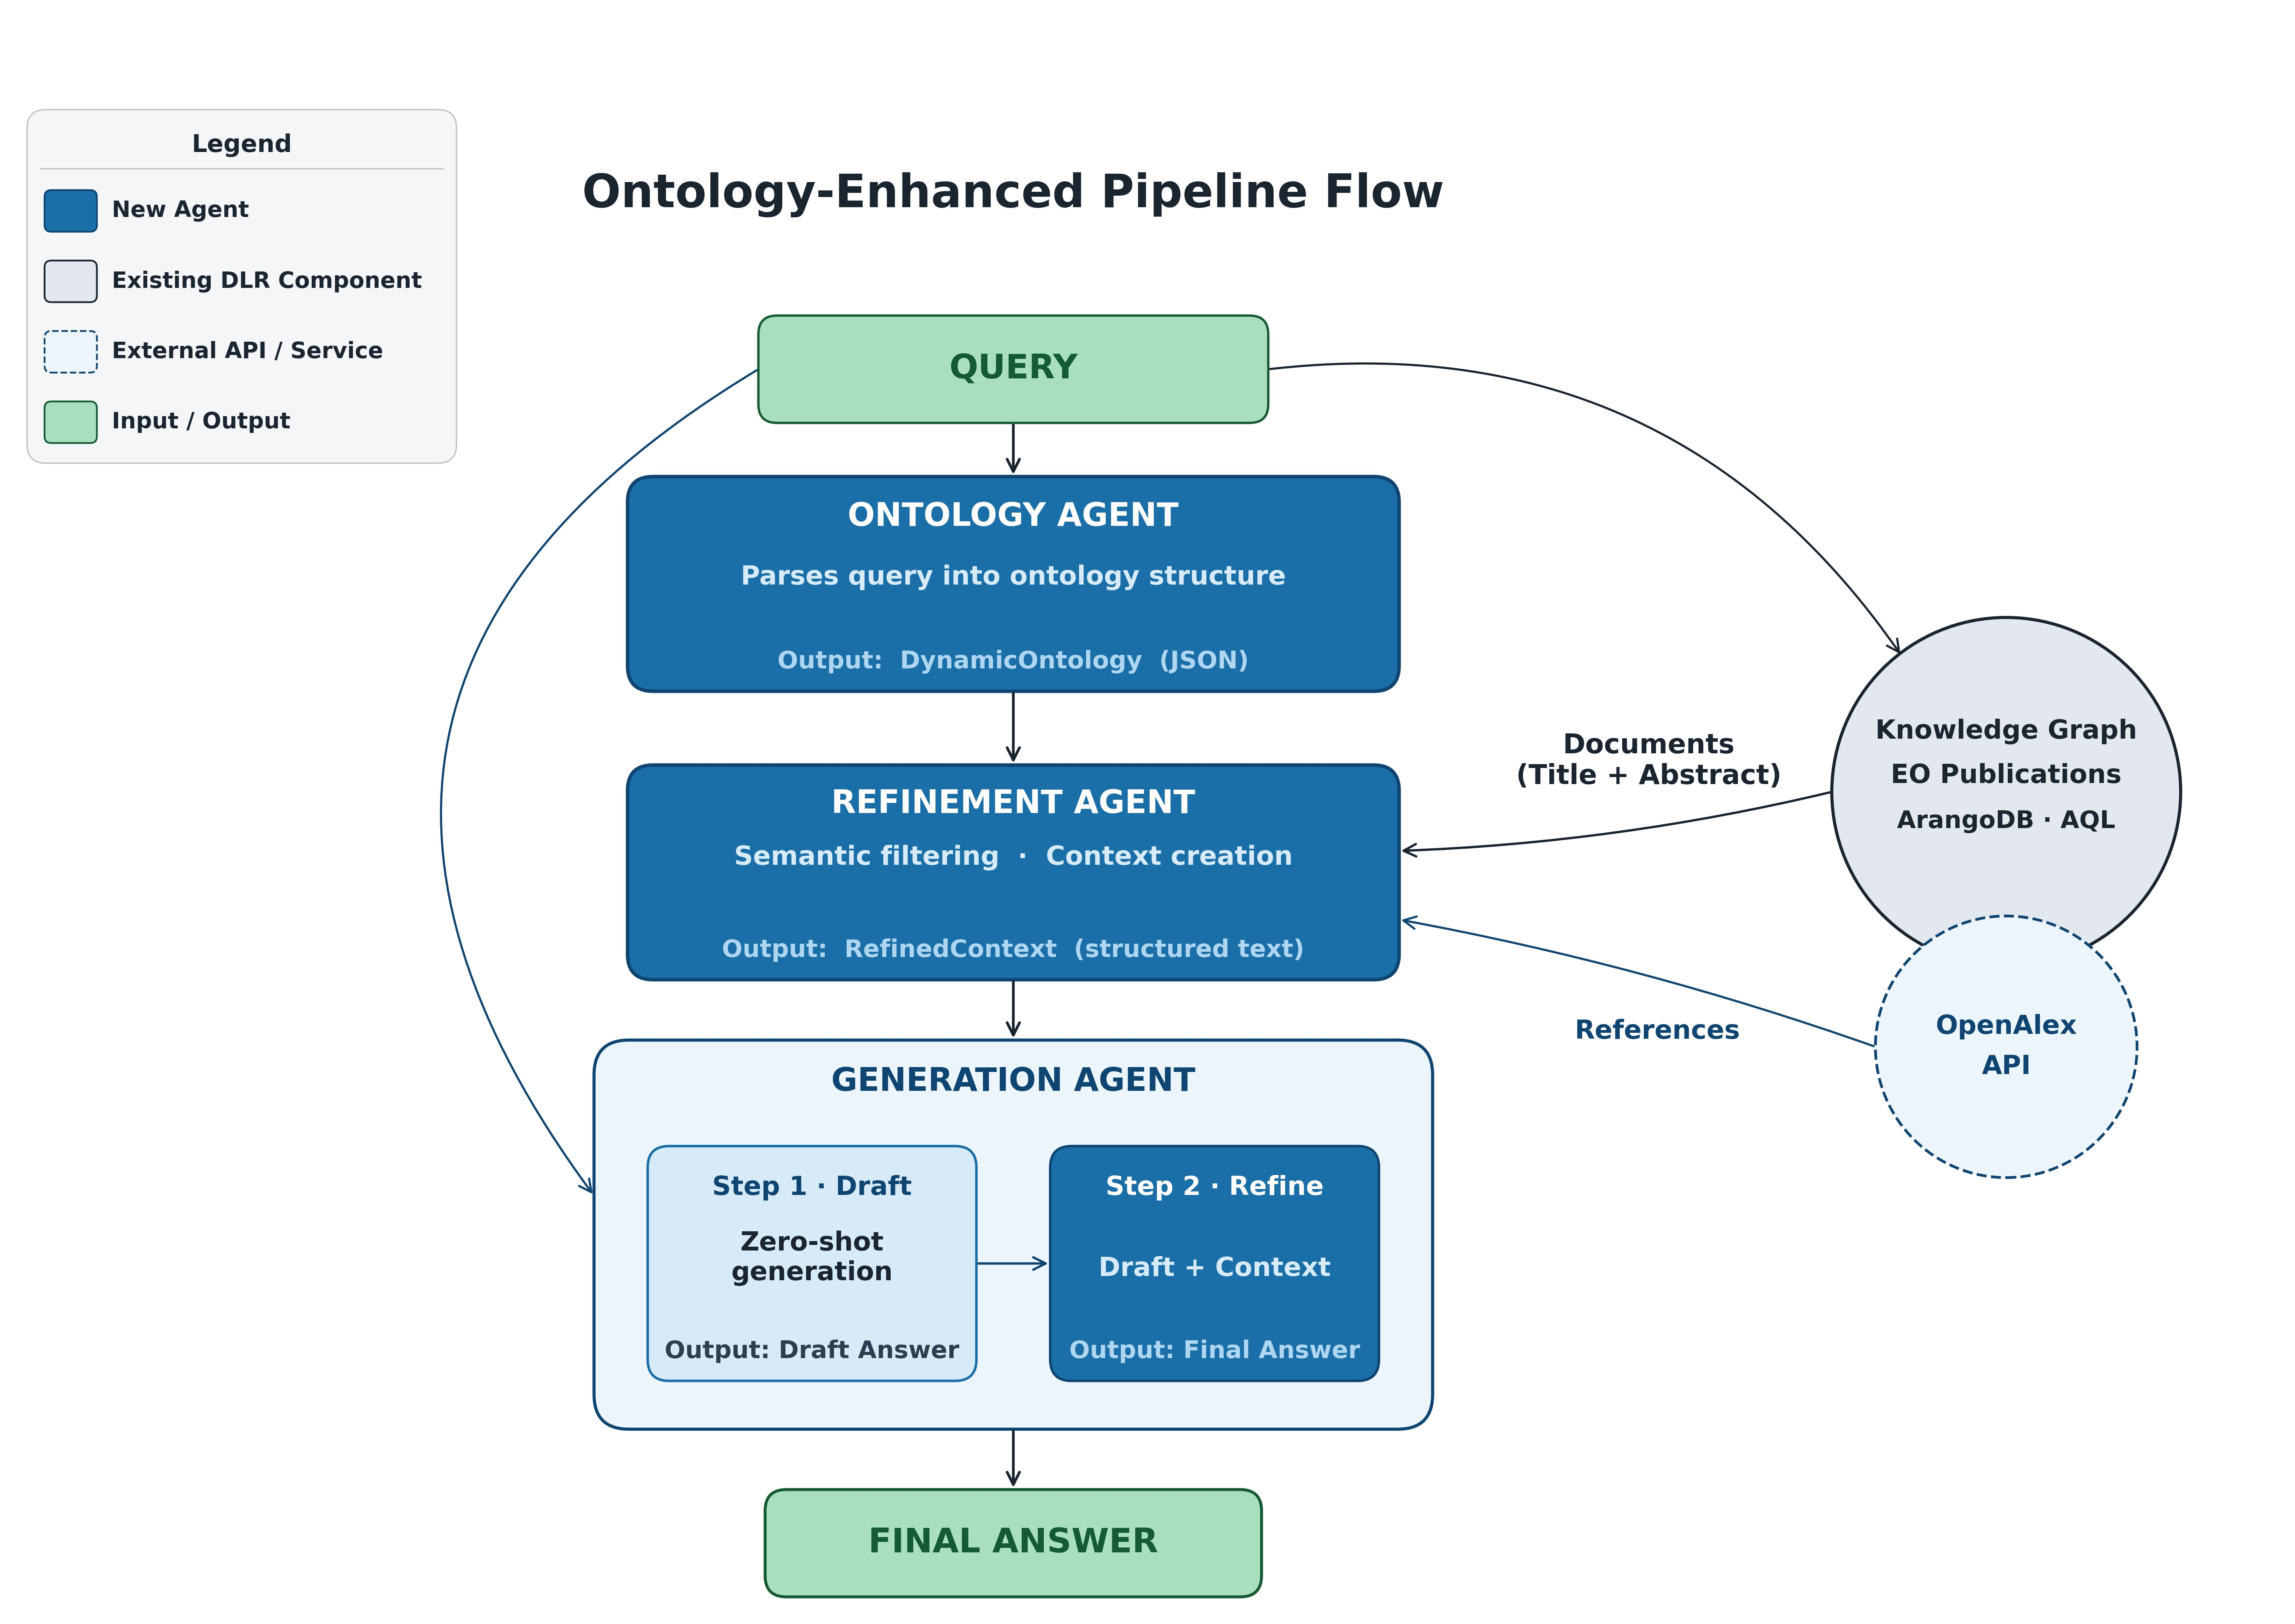
\includegraphics[width=\textwidth]{pipeline_diagram}
\caption{Architecture of the ontology-enhanced multi-agent RAG pipeline. Grey boxes represent existing DLR baseline components; coloured boxes represent the three new agents.}
\label{fig:pipeline}
\end{figure}
Your compile timed out
Your project exceeded the compile timeout limit on our free plan.

Upgrade to get more compile time (plus additional collaborators, document history, track changes, and more).


Command \showhyphens has changed.
‪./bscthesis.tex‬
Reference `lst:prompt-ontology' on page 24 undefined on input line 190.
‪./approach.tex, 190‬
Font shape `OMS/ntxtlf/m/it' undefined
‪./approach.tex‬
Reference `lst:prompt-refinement' on page 27 undefined on input line 333.
‪./approach.tex, 333‬
Reference `lst:prompt-refinement-no-ontology' on page 27 undefined on input line 333.
‪./approach.tex, 333‬
Reference `lst:prompt-generation' on page 30 undefined on input line 441.
‪./approach.tex, 441‬
Underfull \hbox (badness 10000) in paragraph at lines 88--88
‪./bscthesis.tex, 88‬
Underfull \hbox (badness 10000) in paragraph at lines 52--53
‪./introduction.tex, 52‬
Overfull \hbox (20.06451pt too wide) in paragraph at lines 182--183
‪./approach.tex, 182‬
%% ============================================================
\section{Ontology Agent}
\label{sec:ontology-agent}
%% ============================================================

\subsection{Role and Input/Output}
\label{subsec:ontology-role}

The Ontology Agent is the first agent in the pipeline and the only one that works entirely independently of the knowledge graph. In a single LLM call, it takes the user's question and returns a \texttt{DynamicOntology} (schema in Appendix~\ref{app:schema-ontology}): a structured set of typed attribute-value pairs representing the question's semantic requirements. The Refinement and Generation Agents use it for document selection, filtering, and scope-aware generation.

The ontology does not capture every aspect of the question. It captures the dimensions along which evidence is either applicable or not. For the question \textit{``How can above-ground biomass in boreal forests be estimated using Sentinel-1 C-band SAR, and what are the main accuracy limitations?''}, the relevant dimensions are the biophysical variable (AGB), the sensor (C-band SAR), the geographic context (boreal forest), and the accuracy concern (C-band saturation).

\subsection{Ontology Structure}
\label{subsec:ontology-structure}

\subsubsection{Attribute-Value Pairs}
\label{subsubsec:av-pairs}

Each ontology contains 4 to 8 attribute-value pairs. A pair captures one semantic requirement of the question. The fields are: \emph{attribute} (dimension name), \emph{value} (specific concept), \emph{description} (1--2 sentences contextualising the pair for this question), \emph{centrality score}, and optional \emph{constraints} such as units. Listing~\ref{lst:av-pair-example} shows a representative pair.

\begin{lstlisting}[language={}, caption={Example attribute-value pair for the boreal biomass question.}, label={lst:av-pair-example}]

"attribute": "biophysical_variable",
"value": "above_ground_biomass",
"description": "Above-ground biomass density in boreal
forest stands, the primary target variable.",
"centrality": 1.0,
"constraints": ["Mg/ha"]

\end{lstlisting}

\subsubsection{Mandatory Categories}
\label{subsubsec:mandatory-categories}

The prompt requires coverage of at least four of five mandatory dimensions:

\begin{description}
\item[Biophysical variable:] What is being measured (e.g., above-ground biomass, Normalised Difference Vegetation Index (NDVI), sea ice extent).
\item[Sensor/Method:] The observation platform or measurement technique (e.g., Sentinel-2, Synthetic Aperture Radar (SAR) backscatter regression).
\item[Spatial qualifier:] Geographic scope or resolution (e.g., boreal forest, Arctic, 1~km resolution).
\item[Temporal qualifier:] Time period or temporal resolution (e.g., decadal trends, 2000--present).
\item[Application domain:] Scientific purpose (e.g., biomass estimation, climate assessment).
\end{description}

These five dimensions reflect how EO researchers judge whether a piece of evidence is applicable to their question. When a researcher asks about ``boreal SAR biomass,'' they implicitly need documents that match on variable, sensor, and geographic context. The ontology turns these implicit requirements into an explicit, structured representation.

\subsubsection{Centrality Scoring}
\label{subsubsec:centrality-scoring}

Each attribute carries a centrality score indicating how critical it is to the question. We use six discrete levels (Table~\ref{tab:centrality-scale}) rather than a binary accept/reject scale. A binary scale cannot represent partial matches: a document may satisfy a centrality-1.0 attribute while missing a centrality-0.5 one, and that distinction matters for deciding whether to include it.

\begin{table}[htbp]
\centering
\caption{Six-point centrality scale for ontology attributes.}
\label{tab:centrality-scale}
\begin{tabular}{cl}
\toprule
Score & Meaning \\
\midrule
1.0 & \textbf{Absolutely critical:} answer is impossible without this \\
0.9 & \textbf{Core mechanism:} primary driver of the answer \\
0.7 & \textbf{Important enabler:} significantly constrains or enables the answer \\
0.5 & \textbf{Contextual support:} enriches understanding but not essential \\
0.3 & \textbf{Background framework:} contextual framing only \\
0.1 & \textbf{Peripheral:} minimal relevance to the answer \\
\bottomrule
\end{tabular}
\end{table}

Multiple attributes can receive 1.0 or 0.9. Pair count scales with complexity: 4--5 pairs for simple definitional questions, 5--6 for standard causal or comparative questions, and 6--8 for complex multi-mechanism questions.

\subsection{Prompt Design}
\label{subsec:ontology-prompt-design}

The ontology extraction prompt is shown in Listing~\ref{lst:ontology-prompt-excerpt}. Several deliberate design decisions shape its structure.

\begin{lstlisting}[language={}, caption={Key sections of the ontology extraction prompt.}, label={lst:ontology-prompt-excerpt}]
TASK: Extract semantic attributes from Earth Observation questions

Extract 4-8 attribute-value pairs capturing key concepts
essential for answering the question.
Focus on semantic completeness - cover all major scientific
dimensions mentioned.

MANDATORY CATEGORIES (cover >= 4 of 5):
1. BIOPHYSICAL_VARIABLE: What's measured?
2. SENSOR/METHOD: How measured?
3. SPATIAL_QUALIFIER: Where?
4. TEMPORAL_QUALIFIER: When?
5. APPLICATION_DOMAIN: Why?

CENTRALITY SCALE (6-point):
1.0: ABSOLUTELY CRITICAL
0.9: CORE MECHANISM
...

COMPLEXITY TIERS (pair counts are GUIDELINES, not targets):
Simple questions (typically 4-5 pairs)
Standard questions (typically 5-6 pairs)
Complex questions (typically 6-8 pairs)

VALUE SPECIFICITY:
Good: glacier_velocity, NDVI_anomaly, C-band_saturation
Bad: change, data, conditions

SEMANTIC VALIDATION CHECKLIST:
- Does every major scientific concept have an attribute?
- Are all implied measurement methods captured?
- Are geographic and temporal constraints represented?
- Can a domain expert answer using ONLY these pairs?

RETURN ONLY THIS JSON STRUCTURE (valid JSON, no markdown):
{ "pairs": [{ "attribute": ..., "value": ...,
"description": ..., "centrality": ... }] }
\end{lstlisting}

Several design decisions shape the prompt:

\begin{itemize}
\item \textbf{Pair count by complexity.} Three tiers (simple, standard, complex) with suggested pair counts prevent the model from padding simple questions or under-specifying complex ones.
\item \textbf{Category coverage.} At least four of five dimensions must be represented, so the question is broken into distinct scientific aspects~\citep{berant2013semantic} rather than treated as a single query string.
\item \textbf{Specific values.} Contrasting examples (\texttt{glacier\_velocity} vs.\ \texttt{change}) push the model toward values the Refinement Agent can actually match against.
\item \textbf{Strict JSON output.} A fixed schema ensures the response can be parsed directly without post-processing~\citep{bechard2024reducing}.
\item \textbf{Validation checklist.} Before returning, the model checks whether a domain expert could answer the question using only the extracted pairs~\citep{wei2022chain}.
\end{itemize}

The complete prompt is provided in Listing~\ref{lst:ontology-prompt} (Appendix~\ref{app:prompt-ontology}).

\subsection{Example}
\label{subsec:ontology-example}

Table~\ref{tab:ontology-example} shows the ontology generated for the boreal biomass question from Chapter~\ref{chap:preliminaries}.

\begin{table}[htbp]
\centering
\caption{Example ontology for: ``How can above-ground biomass in boreal forests be estimated using Sentinel-1 C-band SAR data, and what are the main accuracy limitations?''}
\label{tab:ontology-example}
\begin{tabular}{clllc}
\toprule
\# & Category & Attribute & Value & Centrality \\
\midrule
1 & Biophysical variable & biophysical\_variable & above\_ground\_biomass & 1.0 \\
2 & Sensor/Method & sensor\_method & Sentinel-1\_C-band\_SAR & 0.9 \\
3 & Spatial qualifier & spatial\_qualifier & boreal\_forest & 0.9 \\
4 & Biophysical variable & accuracy\_limitation & C-band\_saturation & 0.9 \\
5 & Application domain & application\_domain & biomass\_estimation & 0.7 \\
6 & Sensor/Method & estimation\_approach & SAR\_backscatter\_regression & 0.7 \\
7 & Temporal qualifier & temporal\_qualifier & multi-temporal\_analysis & 0.5 \\
\bottomrule
\end{tabular}
\end{table}

The target variable (AGB, 1.0), the specific sensor (Sentinel-1 C-band, 0.9), the geographic constraint (boreal forest, 0.9), and the key accuracy concern (C-band saturation, 0.9) all receive high centrality. The temporal qualifier receives 0.5 because the question does not stress any specific time period.

%% ============================================================
\section{Refinement Agent}
\label{sec:refinement-agent}
%% ============================================================

\subsection{Role and Input/Output}
\label{subsec:refinement-role}

The Refinement Agent sits between knowledge-graph retrieval and answer generation. Its job is to turn raw AQL results into a curated, structured context that the Generation Agent can use directly. It takes three inputs: the user question, the ontology, and the raw AQL documents (title, abstract, URI per document). It returns a plain-text \texttt{enriched\_context} with four labelled sections: an ontology summary, a topics-and-information block, a validated references section, and a caveats-and-gaps section. This output is passed directly to the Generation Agent's prompt without further modification.

In a single LLM call, the agent performs two operations: (1) \emph{selective filtering}, choosing which documents are relevant enough to include, and (2) \emph{structured synthesis}, reorganising selected evidence by topic, tagging each finding with geographic and temporal scope, and attaching per-topic usage instructions. For documents carrying OpenAlex URIs, it also fetches author, year, journal, and DOI metadata via the OpenAlex API to produce complete academic references.

\subsection{Document Assessment}
\label{subsec:document-assessment}

\subsubsection{Partial Relevance}
\label{subsubsec:partial-relevance}

In Earth observation, documents are almost never fully relevant or fully irrelevant. A study of SAR biomass in temperate forests is highly relevant for the sensor and variable dimensions but irrelevant for the spatial qualifier \texttt{boreal\_forest}. Instead of a binary accept/reject filter, the agent evaluates each document along the dimensions defined by the ontology. A document that partially matches is included with an explicit geographic caveat; a document that matches no high-centrality attribute is simply left out of all topics. This is especially important in EO because the literature for any given variable-sensor-region combination is sparse. Excluding all partial matches would often leave the context empty.

\subsubsection{Centrality-Weighted Selection}
\label{subsubsec:centrality-matching}

Ontology attributes are sorted by centrality in descending order before being presented to the model. The prompt tells the model to prefer documents whose titles or opening sentences explicitly mention the highest-centrality attributes. For the boreal biomass query, \texttt{above\_ground\_biomass} (1.0), \texttt{Sentinel-1\_C-band\_SAR} (0.9), and \texttt{boreal\_forest} (0.9) appear at the top of the ontology block. A document about SAR biomass estimation in tropical forests matches the first two but misses the spatial dimension; it may be included with a caveat rather than discarded. Up to 8~documents are selected; if more than 8 match, the most recent are preferred. If fewer than 3 match, all are used and the caveats section records the limited coverage.

\subsection{Usage Guidance}
\label{subsec:usage-guidance}

For each topic in the refined context, a \texttt{Use} field tells the Generation Agent explicitly how to use the evidence:

\begin{description}
\item[Primary evidence:] ``Use as main trend estimate; cite directly.''
\item[Methodological support:] ``Use for methodology only; note study area is temperate Europe.''
\item[Caveated use:] ``Include with geographic caveat; findings are from tropical forests.''
\item[Implicit exclusion:] Documents not assigned to any topic are omitted from the context.
\end{description}

The \texttt{Caveats \& Gaps} section closes the loop by reporting which ontology dimensions are well-supported by the retrieved evidence and which are absent or poorly covered.

\subsection{Prompt Design}
\label{subsec:refinement-prompt-design}

Listing~\ref{lst:refinement-prompt-excerpt} shows the key sections of the refinement prompt. Its design reflects several techniques used in combination.

\begin{lstlisting}[language={}, caption={Key sections of the refinement prompt.}, label={lst:refinement-prompt-excerpt}]
INPUT:
- USER QUESTION: {query}
- ONTOLOGY (target attributes): {ontology}

AQL RESULTS are numbered; scan from 1 to N and use only
the 3-8 most ontology-relevant items.
Prefer items whose title or first 3 sentences explicitly
mention the key ONTOLOGY attributes.
If more than 8 match, choose the 3-8 most recent.

- AQL RESULTS: {aql_results}

GENERAL RULES:
- Use ONLY information from the ONTOLOGY and AQL_RESULTS.
- Do NOT invent numbers, regions, years, methods, citations.
- If something is missing, write "Not available in AQL results".
- Always specify scope (region + time) for quantitative results.
- Clearly separate regional vs global findings.
- Organise topics by concept (matching ontology attributes),
not by document.

OUTPUT FORMAT:
[ONTOLOGY SUMMARY]
Critical attributes found: ...
Supporting attributes found: ...

[TOPICS AND INFORMATION]
...
# Topic name
Findings: 1-2 key findings (quantitative and/or qualitative).
Evidence: Short citation from AQL.
Scope: Geographic: {region} | Temporal: {years}.
Confidence: {0-1} with 1 short reason.
Limitations: 1-2 specific caveats.
Use: Instruction for the answer model.

[VALIDATED REFERENCES]
1. Author et al. (Year). *Title*. URI.
Scope / Key contribution / Limitations / Use.

[CAVEATS & GAPS]
Ontology coverage:
Addressed: ...
Missing or weak: ...
Generation guidance:
Emphasise: 2-3 best-supported concepts.
Caveat: 1-2 concepts requiring qualification.

RE-SCAN FOCUS: Prioritize matches to
QUERY {query} and ONTOLOGY {ontology}
\end{lstlisting}

Several design decisions shape the prompt:

\begin{itemize}
\item \textbf{Filtering.} Only the 3--8 most ontology-relevant documents are kept~\citep{wang2024filco}, directly addressing the missing usage guidance from Section~\ref{sec:generation-context}.
\item \textbf{Organisation by topic.} Findings are grouped by scientific concept rather than listed document by document. Each topic carries scope tags, a confidence estimate, and a use instruction for the Generation Agent.
\item \textbf{Scope tags on numbers.} Every quantitative result must state its geographic and temporal scope, targeting the context-misalignment failure from Section~\ref{subsec:context-misalignment-example}.
\item \textbf{No invented content.} The prompt prohibits making up numbers, regions, or citations. Missing evidence must be flagged rather than filled in~\citep{bechard2024reducing}.
\item \textbf{Re-scan at prompt end.} Re-stating the query and ontology at the very end keeps the selection criteria fresh when the model starts generating~\citep{liu2024lost}.
\item \textbf{No-ontology variant.} For the ablation, the ontology input is replaced with a note that none is provided and the selection criterion changes to ``prefer items directly relevant to the user question.'' Everything else stays identical, so any difference is attributable to the ontology.
\end{itemize}

The complete prompts for both the ontology-enhanced and no-ontology variants are provided in Listings~\ref{lst:refinement-prompt} and~\ref{lst:refinement-prompt-no-ontology} (Appendix~\ref{app:prompt-refinement} and~\ref{app:prompt-refinement-no-ontology}).

%% ============================================================
\section{Generation Agent}
\label{sec:generation-agent}
%% ============================================================

\subsection{Role and Input/Output}
\label{subsec:generation-role}

The Generation Agent turns the curated context from the Refinement Agent into a structured, research-quality answer. Its design is intentionally focused. It refines an existing draft using the structured context from the Refinement Agent. The agent follows the baseline's two-step pattern, extended with an enriched Step~2 prompt. In Step~1, the question alone is sent to the LLM to produce a zero-shot draft. In Step~2, this draft is refined using the structured context from the Refinement Agent, producing a final answer with inline citations and a reference list.

The only change is in the Step~2 prompt. The baseline's Step~2 offered minimal guidance; the revised prompt adds explicit rules for integrating the draft with the context, adapting structure to question type, preserving quantitative scope, and grounding citations.

\subsection{Two-Step Generation}
\label{subsec:two-step-integration}

Step~1 is identical to the baseline: the question is submitted to the LLM without context, and the draft reflects the model's parametric knowledge of the topic. This draft is not shown to the user; it is an internal starting point for the refinement step.

In Step~2, the prompt receives the question, the draft, and the refined context. Five rules govern how the two sources are integrated:

\begin{enumerate}
\item If the draft and context \emph{agree}, keep and optionally enrich.
\item If they \emph{conflict}, align with the context, especially for numbers, regions, and time windows.
\item If important evidence is \emph{in the context but absent from the draft}, add it if it clearly helps answer the question.
\item If material is \emph{in the draft but not in the context}, retain it only if it is standard, well-established background; otherwise remove it or mark it as tentative.
\item When \emph{multiple context items} report related findings, synthesise explicitly (``Several studies show\ldots'') with numeric citations, rather than listing each document separately.
\end{enumerate}

This ordering ensures that retrieved, scope-tagged evidence dominates quantitative claims and geographic context, while the draft contributes general background that the retrieval corpus may not cover. Retrieved, scope-tagged evidence takes priority over parametric knowledge for specifics; parametric knowledge fills in established background~\citep{lewis2020retrieval}.

\subsection{Prompt Design}
\label{subsec:generation-prompt-design}

Listing~\ref{lst:generation-prompt-excerpt} shows the key sections of the generation refinement prompt. The design addresses each of the four failure patterns from Chapter~\ref{chap:preliminaries}.

\begin{lstlisting}[language={}, caption={Key sections of the generation refinement prompt.}, label={lst:generation-prompt-excerpt}]
Most important rules (follow even if other instructions conflict):
- Base all key claims primarily on the provided CONTEXT.
- If draft and CONTEXT conflict, prefer CONTEXT for numbers,
regions, and time windows.
- Do not invent or modify quantitative values that contradict
the CONTEXT.
- Match the complexity and depth of the answer to the question.

### YOUR DRAFT ANSWER
- Question: {question}
- Draft Answer: {draft_answer}
...
### CONTEXT
{context}

RE-SCAN FOCUS: Remember the QUERY {question}

STRUCTURE:
- Begin with a short direct answer (2-4 sentences).
- Then add 2-4 sections with headings matched to question type:
"Key concepts" / "Definition" for 'what is' questions
"Main mechanisms" / "Impacts" for 'how/why' questions
"Comparison of X and Y" for comparison questions
- For comparison questions, include ONE comparison table.
- Add "Uncertainties and limitations" when caveats apply.
- End with "Implications" when modelling or policy relevance
is clear.

USE OF NUMBERS:
- For any quantitative value from CONTEXT, always specify:
* geographic scope (e.g., "Hindu Kush Himalaya, 27-37N")
* temporal scope (e.g., "2000-2024")
- If the question is GENERAL: keep the narrative global;
use regional details only as clearly labelled examples.
- If the question is SPECIFIC to a region: focus there;
use global context only as background.

CITATIONS:
- Insert numeric markers [1], [2] for key claims from CONTEXT.
- Do NOT fabricate or hallucinate references.
- Add a References section at the end using the exact format
from [VALIDATED REFERENCES].

STYLE:
- Do NOT copy internal context headers or pipeline metadata.
- Be informative but not verbose; avoid restating the same
numbers or phrases.
\end{lstlisting}

Several design decisions shape the prompt, each targeting a failure from Chapter~\ref{chap:preliminaries}:

\begin{itemize}
\item \textbf{Important rules first.} Grounding and conflict-resolution rules appear at the very top of the prompt, before any input, so the model reads them first~\citep{liu2024lost}.
\item \textbf{Re-scan between draft and context.} A line re-stating the query sits between the draft and the context block, keeping the question fresh when the model moves into the long context~\citep{liu2024lost}.
\item \textbf{Structure matched to question type.} Comparison questions get a table, causal questions get reasoning steps, definitional questions get a key-concepts section~\citep{wei2022chain}. This replaces the baseline's uniform paragraph format (Section~\ref{subsec:poor-structure-example}).
\item \textbf{Direct opening.} The answer must start with 2--4 sentences that answer the question, targeting the delayed-directness failure (Section~\ref{subsec:delayed-answers-example}).
\item \textbf{Scope on every number.} Every quantitative value must carry its geographic and temporal scope. The Refinement Agent tags them; the Generation Agent must keep those tags.
\item \textbf{Uncertainty where needed.} Caveats from the \texttt{[CAVEATS \& GAPS]} section are carried into the answer, targeting the context-misalignment failure (Section~\ref{subsec:context-misalignment-example}).
\item \textbf{Citations from context only.} References use only entries from the Refinement Agent's \texttt{[VALIDATED REFERENCES]}. Made-up citations are prohibited~\citep{lewis2020retrieval}.
\end{itemize}

The complete generation refinement prompt is provided in Listing~\ref{lst:prompt-generation} (Appendix~\ref{app:prompt-generation}).

%% ============================================================
\section{Pipeline Integration}
\label{sec:pipeline-integration}
%% ============================================================

The three agents integrate into the existing pipeline at clearly defined boundaries. The Ontology Agent is inserted \emph{before retrieval}: it receives the raw question and produces the ontology, but does not modify the AQL query itself. The Refinement Agent is inserted \emph{after retrieval, before generation}: it replaces the baseline's direct forwarding of the parsed original context (presented previously in Section~\ref{sec:generation-context}). The Generation Agent replaces only the Step~2 refinement prompt; Step~1 remains unchanged from the baseline.

A single query uses four LLM calls: one for ontology construction, one for context refinement, and two for generation (draft and refinement). The baseline uses two. Per-query token usage across all agents ranges from 5{,}000 to 7{,}500 tokens, comfortably within the context window of Mistral Small 24B.

%% ============================================================
\section{Expected Improvements}
\label{sec:hypothesis}
%% ============================================================

Based on the failure analysis in Chapter~\ref{chap:preliminaries} and the literature on LLM context utilisation, we expect the largest gains on \textbf{directness} and \textbf{scope awareness}. The prompt improvements target these two criteria most directly: directness through the opening-answer mandate, and scope awareness through the ontology's spatial and temporal qualifiers combined with the Refinement Agent's scope-tagging. As shown in Chapter~\ref{chap:preliminaries}, the baseline's retrieval step actively hurts directness (dropping from 6.67 zero-shot to 4.59 with context), suggesting that structured guidance is needed for retrieval to improve directness rather than degrade it.

We also expect gains on response structure and scientific accuracy. Quantitative precision should improve but will likely remain the hardest criterion, since it depends on whether the source abstracts actually contain specific numbers. We return to this in the results discussion.

The no-ontology variant serves as the primary ablation: if the ontology-enhanced pipeline outperforms it, the improvement is attributable to ontology-guided semantic reasoning rather than to the general prompt improvements both variants share. The next chapter describes the evaluation methodology.
       % Chapters 4: Approach
\chapter{Evaluation Methodology}
\label{chap:evaluation}

\section{Introduction}
\label{sec:eval-intro}

This chapter describes how we evaluate the four pipeline variants introduced in Chapter~\ref{chap:approach}. We use a dataset of 70~Earth observation (EO) questions and a large language model (LLM)-as-a-judge framework with eight criteria scored on a 1--10 scale.

%% ============================================================
\section{Evaluation Dataset}
\label{sec:dataset}
%% ============================================================

\subsection{Question Generation}
\label{subsec:question-generation}

We generated 70~questions using GPT-4.1-mini in a zero-shot manner, combining two axes: a \emph{topic} drawn from the NASA GCMD taxonomy~\citep{nasagcmd2023} and a \emph{question intent} that determines the type of reasoning the question requires. All 14~topics present in the knowledge graph were covered, including atmosphere, cryosphere, and land surface.

Five question intents guide diversity:

\begin{description}
\item[Exploratory:] Discovering new concepts, with no specific expectations. \\ \emph{``How do variations in cryospheric indicators, such as glacier retreat and sea ice extent, influence carbon flux dynamics and land surface heat absorption patterns?''}
\item[Comparative:] Comparing two scientific concepts or methods. \\ \emph{``How do genetic analysis methods compare to traditional physical characteristic-based approaches in classifying vertebrates, invertebrates, and fungi?''}
\item[Descriptive:] Explaining or describing a concept. \\ \emph{``What is the role of climate change adaptation in mitigating risks to human settlements?''}
\item[Causal:] Identifying cause and effect between phenomena. \\ \emph{``How do variations in atmospheric gas concentrations preserved in ice core records influence global temperature changes during glacial and interglacial periods?''}
\item[Relational:] Characterising the relationship between two concepts. \\ \emph{``What is the relationship between cloud cover variability and changes in atmospheric temperature at different altitudes?''}
\end{description}

The combination of 14~topics and 5~intents covers factual recall, method comparison, multi-mechanism causal reasoning, and cross-domain synthesis. These questions are where ontology-guided refinement is expected to matter most: each requires the system to match evidence across several semantic dimensions simultaneously.

%% ============================================================
\section{Pipeline Variants}
\label{sec:pipeline-variants}
%% ============================================================

We compare four pipeline configurations. All use Mistral Small 24B as the generation model.

\begin{description}
\item[Zero-shot baseline.] The question is submitted to Mistral Small without any retrieved context. It serves as a lower bound and makes retrieval degradation visible when it occurs.

\item[Two-step baseline.] The pipeline described by~\citet{elbaff2025earthobservationrag}: a zero-shot draft refined using raw context from the EO knowledge graph. It uses no ontology, no intermediate document assessment, and the original DLR generation prompt.

\item[No-Ontology variant.] This variant uses the same improved Refinement and Generation Agent prompts as the ontology-enhanced pipeline, but the Refinement Agent receives no ontology. It evaluates documents based on the question text alone. This ablation isolates the ontology's contribution from prompt engineering improvements.

\item[Ontology-enhanced pipeline.] The full system described in Chapter~\ref{chap:approach}: ontology construction, ontology-guided refinement, and enhanced generation. This is the primary contribution variant.
\end{description}

%% ============================================================
\section{LLM-as-a-Judge Framework}
\label{sec:llm-as-judge}
%% ============================================================

\subsection{Motivation}
\label{subsec:motivation}

According to~\citet{zheng2023judging}, strong LLM judges achieve over 80\% agreement with human annotators, matching the level of agreement humans reach among themselves. They also identified the main failure modes of LLM-as-a-judge: position bias (preferring answers presented first in pairwise comparisons), verbosity bias (preferring longer answers), and self-enhancement bias (preferring outputs from the same model family as the judge). Our framework design addresses each of these directly.

\subsection{Initial Framework}
\label{sec:initial-framework}

Our initial evaluation used GPT-4.1-mini as the judge with five criteria on a 1--5 scale, following the setup of the two-step baseline~\citep{elbaff2025earthobservationrag}. Two problems emerged. First, score saturation: most answers clustered at 5, leaving too little room to distinguish between pipeline variants. Second, the five criteria borrowed from the baseline (Factuality, Relevance, Groundedness, Helpfulness, and Depth) do not directly measure the qualities this thesis aims to improve: directness, scope awareness, quantitative precision, and structured response organisation.

\subsection{Final Framework}
\label{sec:final-framework}

The final framework replaces GPT-4.1-mini with Claude Sonnet~4.6 (reducing self-enhancement bias) and expands to eight criteria on a 1--10 scale, avoiding the score saturation that limited the initial framework.

\subsubsection{Evaluation Criteria}
\label{subsubsec:criteria}

The eight criteria divide into two groups:

\paragraph{Thesis-specific criteria (four).}
\begin{description}
\item[Directness (1--10):] Does the answer open with a clear, concise response to the core question before elaborating?
\item[Quantitative Precision (1--10):] Are numerical values, units, and their geographic/temporal scope accurately stated?
\item[Response Structure (1--10):] Is the answer organised with appropriate headers, sections, or tables matched to the question type?
\item[Scope Awareness (1--10):] Does the answer correctly scope its claims geographically and temporally, avoiding unqualified generalisations?
\end{description}

\paragraph{General quality criteria (four).}
\begin{description}
\item[Scientific Accuracy (1--10):] Are the scientific claims factually correct?
\item[Relevance (1--10):] Does the answer address what the question actually asks?
\item[Completeness (1--10):] Does the answer cover the main dimensions of the question?
\item[Helpfulness (1--10):] Is the answer practically useful to someone researching the topic?
\end{description}

The four thesis-specific criteria above were not part of the initial GPT-4.1-mini framework (Appendix~\ref{app:initial-criteria}). Full score-band descriptions for all eight criteria are given in Appendix~\ref{app:eval-criteria}.

The average inter-criterion Pearson correlation across all 280~evaluations is $r = 0.65$. This means that a better answer tends to score higher on multiple dimensions at the same time. An answer that misaligns context (low Scope Awareness) is also likely to be less helpful and less scientifically accurate. The moderate correlation does not undermine the criteria's usefulness: the goal is to identify \emph{where} a pipeline improves, not to treat each dimension as independent.

\subsection{Evaluation Protocol}
\label{subsec:eval-protocol}

For each question-answer pair, the judge receives the system prompt with criteria definitions and score range descriptions, followed by the question and the answer. It returns eight integer scores. Each pair is evaluated on its own. This single-answer grading approach avoids position bias~\citep{zheng2023judging}.

We compute per-pipeline means for each criterion and for the overall score. Per-question score distributions are used for significance testing and per-question analysis.

\subsection{Bias Mitigations}
\label{subsec:bias-mitigations}

No automated evaluation framework removes all biases. The LLM-as-a-judge approach carries the judge model's own biases, and Claude Sonnet~4.6 may not score responses the same way a human EO domain expert would. Although the Directness criterion penalises unnecessary length, some residual verbosity bias likely remains: the ontology-enhanced pipeline produces longer answers on average, and the judge may reward that length independently of informational content. We address this remaining limitation through complementary qualitative error analysis in Chapter~\ref{chap:results}, where we manually inspect the outputs to the four questions from the problem analysis (Section~\ref{sec:failure-patterns}) to verify that score differences correspond to observable quality differences.

%% ============================================================
\section{Significance Testing}
\label{sec:significance-testing}
%% ============================================================

\subsection{Choice of Test}
\label{subsec:test-choice}

We use the Wilcoxon signed-rank test~\citep{wilcoxon1945individual} for all pairwise comparisons between pipeline variants. Three properties of our data make it the right choice. Scores are ordinal integers on a 1--10 scale, and the Wilcoxon test requires no normality assumption. The 70~questions are evaluated under all four pipeline variants, so the scores are paired: each question serves as its own control, removing question-level variance from the comparison. The Wilcoxon test is also more powerful than the sign test while remaining distribution-free, relevant given the sample of 70~questions.

\subsection{Correction for Multiple Comparisons}
\label{subsec:multiple-comparisons}

We perform six pairwise comparisons (the number of pairs from four pipeline variants) for each of the eight criteria. We apply Bonferroni correction within each criterion: $\alpha = 0.05$ divided across six pairwise comparisons gives $\alpha_{\text{corrected}} = 0.0083$ per test. Across all eight criteria, this amounts to 48 individual tests. When a corrected $p$-value falls below this threshold, we report the difference as statistically significant.

\subsection{Effect Size}
\label{subsec:effect-size}

A significant result does not mean the difference matters in practice, especially with 70~paired observations where the test has enough power to flag even small differences as significant. We therefore report an effect size estimate for each significant finding using the rank-biserial correlation $r$, calculated from the Wilcoxon test statistic~\citep{kerby2014simple}. We interpret $r \geq 0.1$ as small, $r \geq 0.3$ as medium, and $r \geq 0.5$ as large. We report results as significant only when both the corrected $p$-value and the effect size meet their respective thresholds.
       % Chapters 5: Evaluation Methodology
\chapter{Results and Analysis}
\label{chap:results}

% =============================================================================
\section{Chapter Overview}
\label{sec:results-overview}
% =============================================================================

This gives 280~evaluations (70~questions $\times$ 4~pipelines) and 2{,}240 individual criterion scores. An earlier round using GPT-4.1-mini as judge is reported in Section~\ref{sec:initial-framework}; the Claude-based evaluation is the primary evidence base.

% =============================================================================
\section{Overall Pipeline Performance}
\label{sec:overall-performance}
% =============================================================================

\begin{table}[htbp]
\centering
\caption{Overall pipeline ranking on the 70-question EO benchmark, evaluated
by Claude Sonnet~4.6 (mean of eight criteria, 1--10 scale). The ontology-enhanced
pipeline leads on all criteria; the two-step baseline finishes last.}
\label{tab:overall-ranking}
\begin{tabular}{clcl}
\toprule
\textbf{Rank} & \textbf{Pipeline} & \textbf{Overall Score} & \textbf{Note} \\
\midrule
1 & Ontology-Enhanced RAG & 7.48 / 10 & Best \\
2 & No-Ontology RAG & 6.88 / 10 & Second \\
3 & Zero-Shot & 6.28 / 10 & Third overall \\
4 & Two-Step RAG Baseline & 5.51 / 10 & Lowest overall \\
\bottomrule
\end{tabular}
\end{table}

\begin{figure}[htbp]
\centering
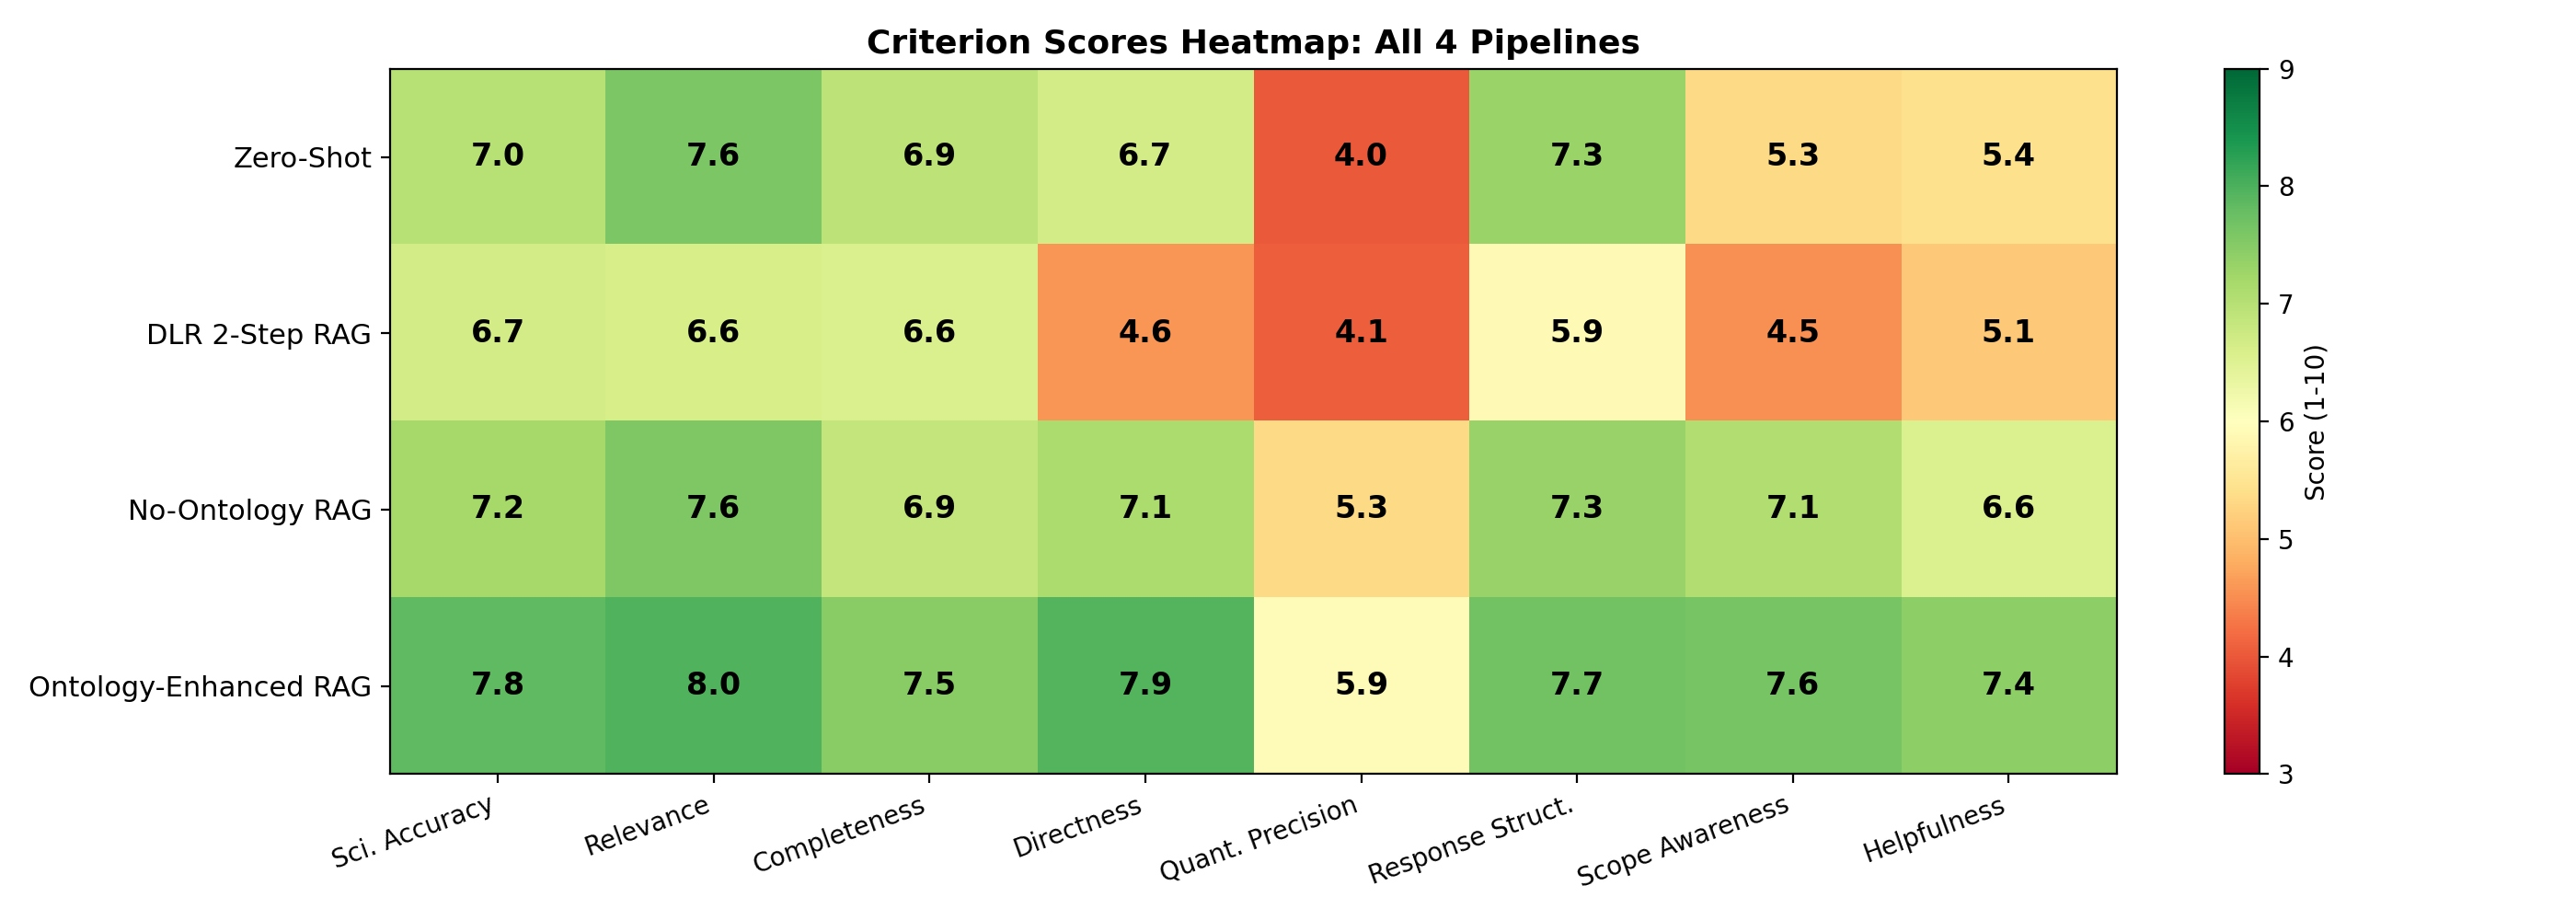
\includegraphics[width=0.85\textwidth]{chart_4pipe_heatmap.jpg}
\caption{Heatmap of mean criterion scores across all four pipelines. The ontology-enhanced pipeline (top row) leads on every criterion; quantitative precision forms a distinct cool band across all pipelines, reflecting the abstract-only data limitation.}
\label{fig:heatmap-overview}
\end{figure}

Table~\ref{tab:overall-ranking} shows the full ranking. The gaps between consecutive pipelines are roughly even: +0.60 from no-ontology to ontology, +0.60 from zero-shot to no-ontology, and +0.77 from the two-step baseline to zero-shot.

A notable result is that the two-step baseline (5.51) scores below the zero-shot baseline (6.28). The context and generation-agent prompts in the two-step baseline degrade the final answers. This is not driven by a few outliers: the two-step baseline underperforms zero-shot on 66 of 70~questions. Per criterion, directness drops by 2.09 points, response structure by 1.40, relevance by 0.96, and scope awareness by 0.80. The only criterion where the two-step baseline slightly beats zero-shot is quantitative precision (+0.06), which is negligible. These drops map directly onto the four shortcomings from Chapter~\ref{chap:preliminaries}: delayed direct answers, poor structure, relevance drift from context padding, and uncaveated claims.

Their overall scores are close (6.28 vs 6.88), and on several criteria the differences are small: relevance (7.57 vs 7.56), completeness (6.91 vs 6.86), and scientific accuracy (7.00 vs 7.19). The improved refinement and generation prompts alone, without the ontology, bring performance back to roughly the zero-shot level on core quality metrics. The bigger differences appear on scope awareness (5.34 vs 7.07) and helpfulness (5.41 vs 6.56), where the restructured pipeline already helps. The ontology-enhanced variant pulls clearly ahead on all eight criteria, so ontology-guided semantic reasoning adds a consistent edge that prompt improvements alone do not reach.

The heatmap in Figure~\ref{fig:heatmap-overview} shows the same pattern visually. The gap between the ontology-enhanced and no-ontology variants is smaller than the gap between the two-step baseline and zero-shot. The three-agent architecture with structured refinement accounts for the larger share of the improvement; the ontology adds a further consistent increment on top.

% =============================================================================
\section{Per-Criterion Analysis}
\label{sec:per-criterion}
% =============================================================================

\begin{table}[htbp]
\centering
\caption{Mean scores per criterion for each pipeline (1--10 scale).
Bold values mark the highest score in each criterion column. Directness
shows the largest single-criterion gap (7.93 vs 4.59); quantitative precision
remains the universal weak spot.}
\label{tab:per-criterion-means}
\small
\begin{tabular}{lcccccccc}
\toprule
\textbf{Pipeline} & \textbf{Sci.Acc} & \textbf{Relev} & \textbf{Compl}
& \textbf{Direct} & \textbf{Quant} & \textbf{Struct}
& \textbf{Scope} & \textbf{Help} \\
\midrule
Zero-Shot & 7.00 & 7.57 & 6.91 & 6.67 & 4.01 & 7.30 & 5.34 & 5.41 \\
Two-Step Baseline & 6.66 & 6.61 & 6.57 & 4.59 & 4.07 & 5.90 & 4.54 & 5.13 \\
No-Ontology & 7.19 & 7.56 & 6.86 & 7.11 & 5.33 & 7.33 & 7.07 & 6.56 \\
Ontology-Enh. & \textbf{7.83} & \textbf{7.96} & \textbf{7.46}
& \textbf{7.93} & \textbf{5.93} & \textbf{7.67}
& \textbf{7.63} & \textbf{7.41} \\
\bottomrule
\end{tabular}
\end{table}

Table~\ref{tab:per-criterion-means} breaks down the scores by criterion. We group the eight criteria into three clusters based on what they measure.

\paragraph{Thesis-critical criteria.} These four criteria correspond directly to the four shortcomings identified in Chapter~\ref{chap:preliminaries}. Directness shows the largest single-criterion gap: the ontology-enhanced pipeline scores 7.93 compared to 4.59 for the two-step baseline, a 3.34-point difference. The ontology gives the generation agent a clear priority order of concepts, so the answer opens with the core mechanism instead of burying it. Scope awareness follows a similar pattern: 7.63 vs 4.54 (a 3.09-point gap). The ontology's spatial and temporal qualifiers (e.g.\ \texttt{polar\_regions}, \texttt{2000--2023}) are passed to the generation agent, which uses them to scope its claims. Response structure improves by 1.77 points (7.67 vs 5.90). The structured refinement output (Topics \& Information, Validated References, Caveats \& Gaps) gives the generation agent pre-organised input that maps onto better-organised answers. Quantitative precision improves by 1.86 points (5.93 vs 4.07), but it remains the weakest criterion for all pipelines. We return to this in Section~\ref{sec:quant-precision}.

\paragraph{Core quality criteria.} Scientific accuracy, relevance, and completeness represent general answer quality. The ontology-enhanced pipeline leads on all three: scientific accuracy at 7.83, relevance at 7.96 (the highest single score of any criterion for any pipeline), and completeness at 7.46. An interesting pattern is that zero-shot relevance (7.57) is nearly identical to no-ontology relevance (7.56). Retrieval on its own does not improve relevance; the ontology's semantic alignment is what pushes it to 7.96 (+0.40). On completeness, the ontology ensures that each semantic dimension (sensors, variables, scope) is addressed, raising the score from 6.86 to 7.46.

\paragraph{Helpfulness.} The ontology-enhanced pipeline scores 7.41 on helpfulness, compared to 6.56 for no-ontology (+0.86, the largest ontology gain). Helpfulness correlates strongly with quantitative precision ($r = 0.80$), so the ontology's ability to surface specific numbers and datasets is what drives perceived usefulness. The two-step baseline (5.13) is only slightly below zero-shot (5.41) on helpfulness despite being worse overall. The judge may still reward the extra context, even when it is poorly structured.

% =============================================================================
\section{Score Distributions and Win Rates}
\label{sec:distributions}
% =============================================================================

\begin{figure}[htbp]
\centering
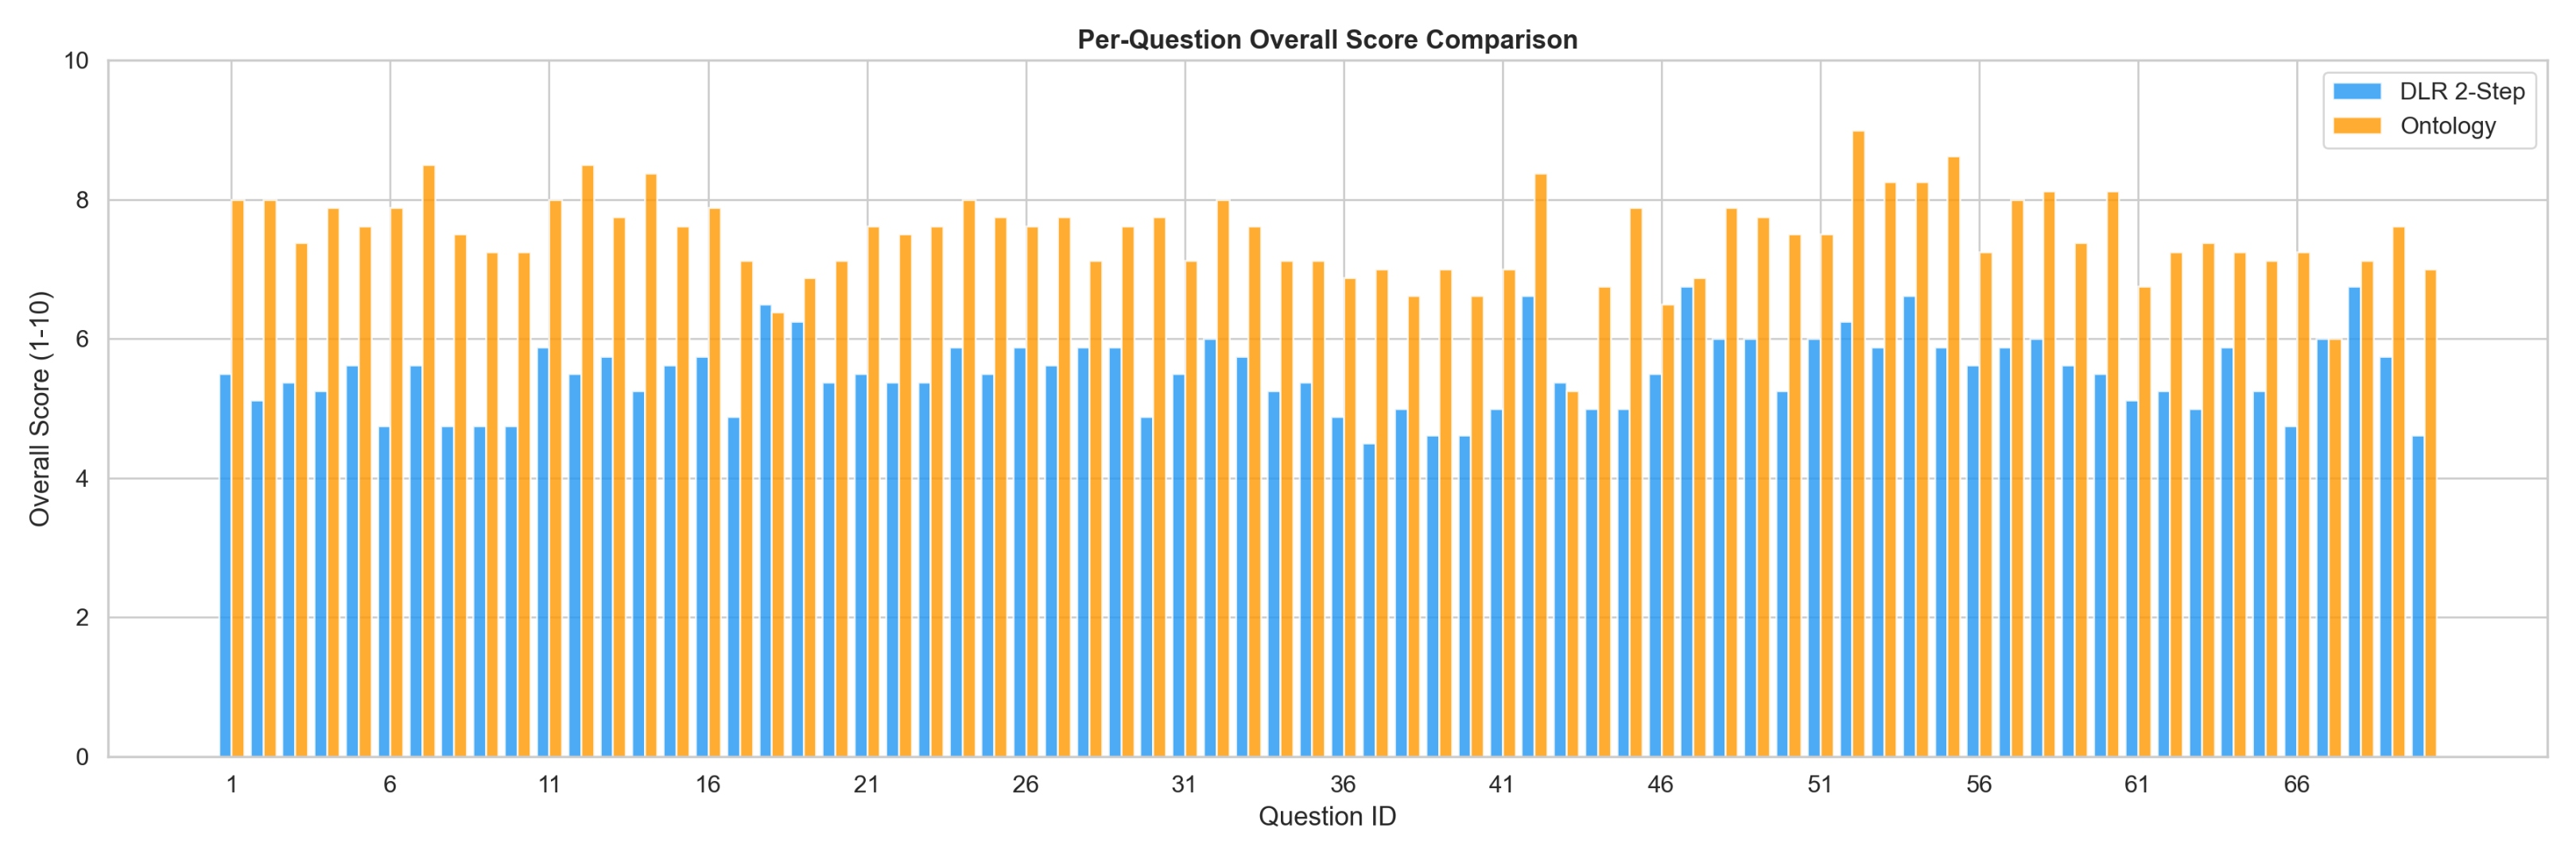
\includegraphics[width=\textwidth]{chart_per_question.jpg}
\caption{Per-question overall scores for the baseline and ontology-enhanced pipelines across the
70-question benchmark, sorted by question index. The ontology-enhanced
pipeline (orange bars) exceeds the baseline pipeline (blue bars) over the full question distribution (with the exception of two questions).}
\label{fig:per-question}
\end{figure}

The ontology-enhanced pipeline wins on 56 of 70~questions (80\%) against the no-ontology variant. The average winning margin is about 0.60 points, with individual margins from under 0.25 (near-ties) to over 1.50 (clear ontology dominance). The largest gains appear on multi-part comparison questions, where the ontology's structured dimensions help the generation agent organise parallel comparisons, and on questions that require explicit spatial or temporal scoping, where the scope qualifiers translate directly into caveats. The 14~questions where the no-ontology variant ties or wins tend to be simpler factual questions, where the ontology adds context overhead with little informational benefit.

On the other end, the two-step baseline loses to zero-shot on 66 of 70~questions (94\%). As Figure~\ref{fig:per-question} shows, the two-step baseline bars sit consistently below the zero-shot bars, with only 4~questions where the two-step baseline marginally exceeds zero-shot (all by less than 0.5 points). The degradation from the two-step refinement is systematic, not driven by a few bad cases.

% =============================================================================
\section{Statistical Significance and Effect Sizes}
\label{sec:statistical}
% =============================================================================

\begin{figure}[htbp]
\centering
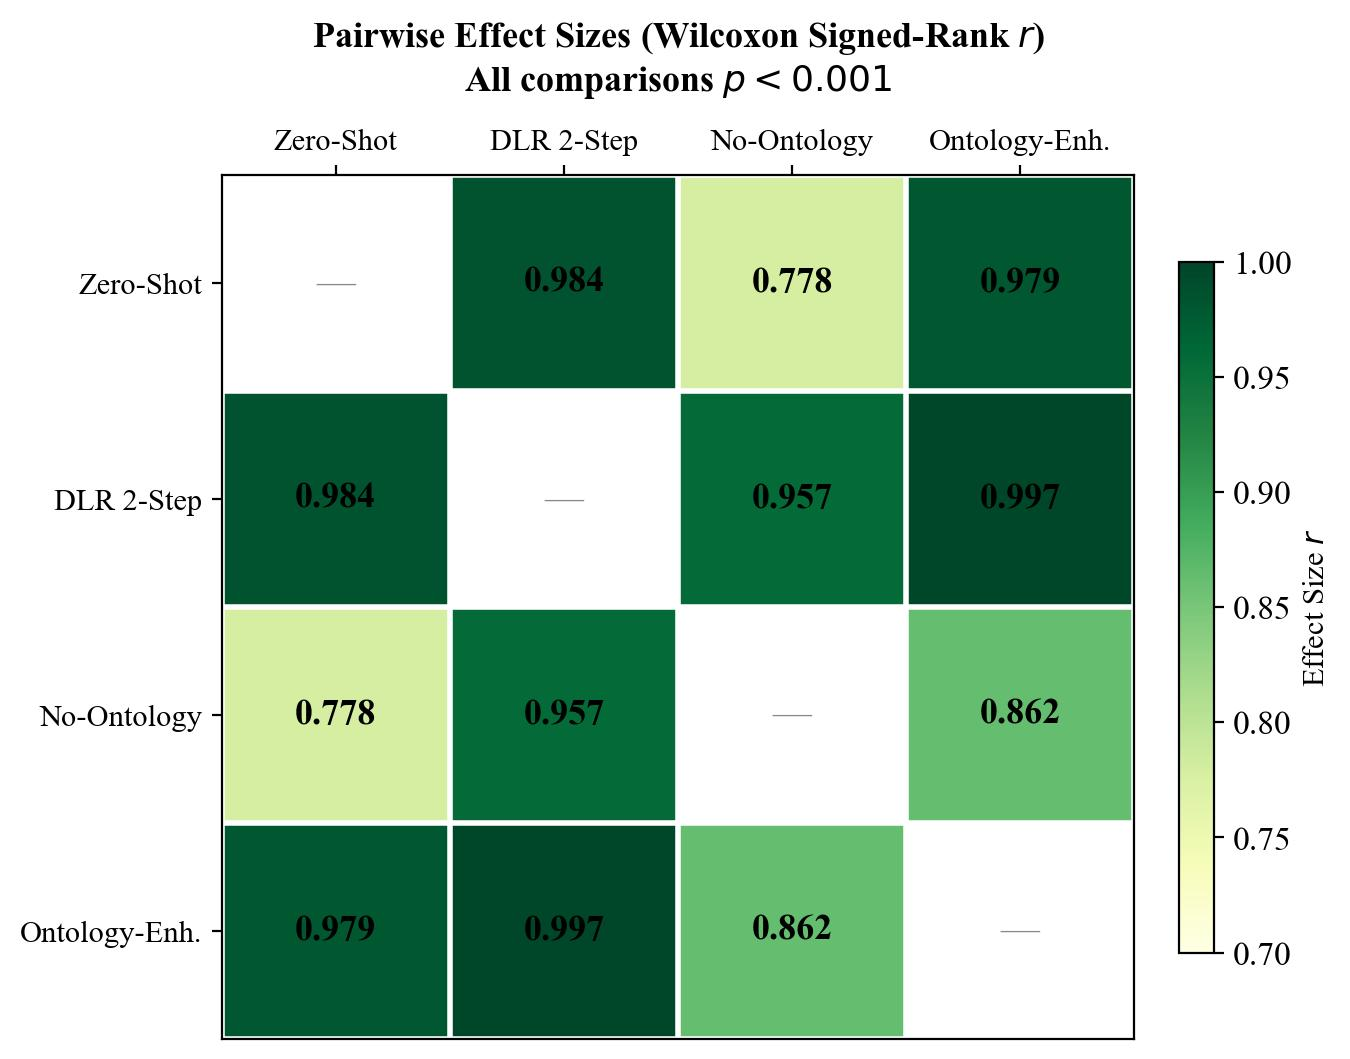
\includegraphics[width=0.75\textwidth]{effect_heatmap.jpg}
\caption{Pairwise effect-size heatmap (Wilcoxon signed-rank $r$) for all
six pipeline comparisons. All effect sizes exceed $r = 0.77$, indicating
large practical differences. The largest effect ($r = 0.997$) is between
the two-step baseline and the ontology-enhanced pipeline; the smallest
($r = 0.778$) is between zero-shot and the no-ontology variant.}
\label{fig:effect-heatmap}
\end{figure}

\begin{table}[htbp]
\centering
\caption{Pairwise Wilcoxon signed-rank tests on per-question overall scores
($n = 70$). All comparisons are significant at $p < 0.001$, with all
effect sizes above $r = 0.77$ (large per~\citet{kerby2014simple}). Effect
sizes ($r$) are computed as $r = Z / \sqrt{N}$.}
\label{tab:pairwise-tests}
\begin{tabular}{llcc}
\toprule
\textbf{Comparison} & \textbf{Direction} & $\boldsymbol{p}$ & \textbf{Effect size} $\boldsymbol{r}$ \\
\midrule
Two-Step vs Ontology & Ontology $\gg$ Two-Step & $< 0.001$ & 0.997 \\
ZS vs Two-Step & ZS $>$ Two-Step & $< 0.001$ & 0.984 \\
ZS vs Ontology & Ontology $\gg$ ZS & $< 0.001$ & 0.979 \\
Two-Step vs No-Ontology & No-Ont $\gg$ Two-Step & $< 0.001$ & 0.957 \\
No-Ont vs Ontology & Ontology $>$ No-Ont & $< 0.001$ & 0.862 \\
ZS vs No-Ontology & No-Ont $>$ ZS & $< 0.001$ & 0.778 \\
\bottomrule
\end{tabular}
\end{table}

\begin{table}[htbp]
\centering
\caption{Per-criterion comparison between the ontology-enhanced and
no-ontology pipelines. All eight criteria show statistically significant
improvements; seven at $p < 0.001$ and one (response structure) at
$p = 0.003$.}
\label{tab:ont-vs-noont-criteria}
\small
\begin{tabular}{lcccl}
\toprule
\textbf{Criterion} & \textbf{No-Ont} & \textbf{Ontology} & \textbf{Diff}
& $\boldsymbol{p}$ \\
\midrule
Helpfulness & 6.56 & 7.41 & +0.86 & $< 0.001$ \\
Directness & 7.11 & 7.93 & +0.81 & $< 0.001$ \\
Scientific Accuracy & 7.19 & 7.83 & +0.64 & $< 0.001$ \\
Completeness & 6.86 & 7.46 & +0.60 & $< 0.001$ \\
Quant.\ Precision & 5.33 & 5.93 & +0.60 & $< 0.001$ \\
Scope Awareness & 7.07 & 7.63 & +0.56 & $< 0.001$ \\
Relevance & 7.56 & 7.96 & +0.40 & $< 0.001$ \\
Response Structure & 7.33 & 7.67 & +0.34 & $= 0.003$ \\
\bottomrule
\end{tabular}
\end{table}

All six pairwise comparisons between pipelines are significant at $p < 0.001$ using the Wilcoxon signed-rank test, with Bonferroni correction applied as described in Chapter~\ref{chap:evaluation}. All effect sizes exceed $r = 0.77$, well above the conventional large threshold of $r = 0.50$. The largest effect ($r = 0.997$) separates the two-step baseline from the ontology-enhanced pipeline, the two endpoints of the ranking. The smallest ($r = 0.778$) separates zero-shot from the no-ontology variant, the two middle-ranked pipelines. Figure~\ref{fig:effect-heatmap} and Table~\ref{tab:pairwise-tests} show these results.

Table~\ref{tab:ont-vs-noont-criteria} focuses on the ontology vs no-ontology comparison per criterion. All eight criteria show significant ontology gains. Response structure shows the smallest gain, since the no-ontology pipeline already benefits from the structured refinement output format.

% =============================================================================
\section{Quantitative Precision: A Universal Weakness}
\label{sec:quant-precision}
% =============================================================================

Quantitative precision is the lowest-scoring criterion for every pipeline: zero-shot scores 4.01, the two-step baseline 4.07, no-ontology 5.33, and the ontology-enhanced pipeline 5.93. The gap between quantitative precision and the overall score is 1.4--2.3 points for every pipeline, a consistent underperformance relative to other criteria. The ontology does improve quantitative precision significantly (+0.60 over no-ontology, $p < 0.001$; +1.92 over zero-shot), but even the best pipeline stays below the 6-point mark.

The main cause is that the knowledge graph currently contains only document abstracts. Abstracts summarise findings in general terms and rarely include exact numbers, specific measurements, or detailed statistics. The full-text sections where those values appear (results tables, figure captions, and method descriptions) are not available to the pipeline. Even when the ontology's centrality scores tell the refinement agent that quantitative detail should exist for a given topic, the source documents do not contain the numbers to extract. Mistral Small can reproduce numerical values when they appear in the input context, but it cannot generate accurate domain-specific numbers from its training data alone. The next chapter discusses how full-text indexing or structured data extraction could address this.

% =============================================================================
\section{Manual Failure Mode Analysis}
\label{sec:failure-mode-analysis}
% =============================================================================

The scores reported above measure aggregate performance across 70~questions. To check whether the ontology-enhanced pipeline actually addresses the four specific failure modes from Chapter~\ref{chap:preliminaries}, we manually inspected the answers to the same four questions that originally exposed those failures.

\paragraph{Delayed direct answers (\S\ref{subsec:delayed-answers-example}).} The original baseline answer to a question about vegetation health sensors spent roughly 600~words on spectral analysis and vegetation indices before naming a single sensor. The ontology-enhanced answer opens with: ``Optical satellite sensors are the primary tools for vegetation health monitoring, using visible, near-infrared (NIR), and shortwave infrared (SWIR) bands to derive indices such as NDVI, EVI, and FAPAR.'' The answer is in the first sentence. The labelled sections that follow (Optical Sensors, Microwave Sensors, Multi-Sensor Fusion) build outward from this core rather than toward it. The ontology's priority order of concepts tells the generation agent that the sensor itself should lead. This is consistent with the directness score improvement from 4.59 to 7.93.

\paragraph{Missing quantitative precision (\S\ref{subsec:missing-precision-example}).} The baseline produced vague, hedge-heavy statements about sensor limitations without citing specific thresholds. The ontology-enhanced answer structures the same comparison as a table with concrete attributes (spectral bands, spatial resolution, cloud sensitivity) side by side. A comparison question now receives a comparative format. However, some table cells still use qualitative descriptors (``saturation at high biomass'') without specifying at what level saturation occurs. The source abstracts often do not contain these numbers, the same data limitation discussed in Section~\ref{sec:quant-precision}. Chapter~\ref{chap:discussion} discusses this further.

\paragraph{Poor response structure (\S\ref{subsec:poor-structure-example}).} The baseline interleaved GEDI and Sentinel-1 information across paragraphs without clear separation when asked to compare the two sensors for boreal forest monitoring. The ontology-enhanced answer separates sensor descriptions into labelled bullet-point lists and adds an application comparison table with rows for canopy height mapping, aboveground biomass, wetland inundation, and temporal monitoring. Each row has columns for GEDI, Sentinel-1, and combined use. A reader can go directly to the attribute they care about and see both sensors side by side. The structured refinement output (Topics \& Information, Validated References, Caveats \& Gaps) gives the generation agent pre-organised material that maps naturally to this kind of layout.

\paragraph{Context misalignment (\S\ref{subsec:context-misalignment-example}).} This was the most critical failure. The baseline reported accuracy values from a study on Japanese temperate coniferous forests as if they applied to boreal forests, without any geographic caveat. The ontology-enhanced answer opens with an explicit scope qualifier (``in coniferous forests'') and includes an Uncertainties and Limitations section that states: ``There are few direct, circumpolar boreal comparisons of GEDI versus Sentinel-1 AGB accuracy; most evidence comes from temperate or plantation coniferous forests, so boreal-specific performance must be inferred cautiously.'' The Japanese study still appears in the references, but its geographic context is now explicit rather than silently assumed to generalise. The ontology's spatial scope qualifiers are what enable this: they give the generation agent what it needs to caveat its claims. The scope awareness improvement from 4.54 to 7.63 reflects this gain.
        % Chapter 6: Results and Analysis
\chapter{Discussion}
\label{chap:discussion}

\section{Overview}
\label{sec:discussion-overview}

Chapter~\ref{chap:results} reported the quantitative results of the four-pipeline comparison. This chapter interprets what those results mean. We discuss why prompt improvements alone are not enough to close the quality gap, how knowledge graph data can be used more effectively, how the approach may transfer to other domains, and where the pipeline falls short. Chapter~\ref{chap:conclusion} then answers each research question and outlines future work.


\section{Why Prompt Changes Are Not Enough}
\label{sec:discuss-prompts}

The no-ontology pipeline and the two-step baseline both retrieve from the same knowledge graph. The difference is that the no-ontology variant uses improved prompts for refinement and generation, organised around the three-agent design with structured output (Topics \& Information, Validated References, Caveats \& Gaps). This gives it a 1.37-point advantage over the two-step baseline (6.88 vs 5.51), which is a large improvement. Prompt changes clearly help. They fix the structural and directness problems that the two-step baseline's raw context injection causes. But the no-ontology pipeline is only marginally better than zero-shot on core quality metrics: relevance is 7.56 vs 7.57 and completeness is 6.86 vs 6.91. The improved prompts recover what bad context processing destroyed, but they do not push quality beyond what the model can already produce on its own.

The ontology adds something that prompt tuning cannot: a query-specific semantic structure that tells the refinement agent what to look for in the documents, and tells the generation agent what dimensions to cover in the answer. Without the ontology, the refinement agent has to decide on its own which parts of the context are relevant to the query. With the ontology, it has a checklist: does this document address the biophysical variable? The sensor? The spatial scope? This is what produces the additional +0.60 on top of the already-improved pipeline. The largest gains are on helpfulness (+0.86) and directness (+0.81), which are the criteria where knowing what matters most makes the biggest difference. As~\citet{liu2024lost} showed, even well-prompted models lose information in long contexts. The ontology acts as an anchor that prevents this by marking what is important before the context is even constructed. In short, prompts change how the model processes context; the ontology changes what context the model gets to process.


\section{Making Use of Knowledge Graph Data}
\label{sec:discuss-kg-data}

The main lesson from the results is that context quality matters more than context quantity. The two-step baseline provides shorter context (about 2{,}948 characters on average) but in unstructured form, and the answers are worse than zero-shot. The three-agent pipeline provides longer context (about 9{,}400--9{,}600 characters) but in structured form, and the answers are better. The knowledge graph built by~\citet{elbaff2025earthobservationrag} is a strong retrieval source. The AQL queries return relevant documents. The problem was never what gets retrieved, but what happens after retrieval: how the context is filtered, organised, and presented to the generation model. This is a general insight for any RAG system built on a knowledge graph. The graph gives you relevant data, but the pipeline has to structure that data around the query's specific needs before passing it to the generator.

One concrete data limitation is that the knowledge graph currently indexes only document abstracts. Abstracts summarise findings in general terms and rarely include exact measurements or detailed statistics. This is the main reason quantitative precision is low across all four pipelines (4.01--5.93). The ontology helps to some extent: centrality scores flag when quantitative detail should exist for a given topic, prompting the refinement agent to look for it. But if the numbers are not in the abstracts, the pipeline cannot surface them. Indexing full-text sections, especially results tables and method descriptions, would give the pipeline access to the specific numbers it currently lacks. This is a data change rather than a pipeline change; the architecture is already ready for richer input.


\section{Applicability Beyond Earth Observation}
\label{sec:discuss-generalisability}

The ontology agent is dynamic: it generates a new ontology for each query rather than relying on a pre-built, fixed ontology. The five semantic dimensions we use for EO (biophysical variable, sensor/method, spatial scope, temporal scope, application domain) are one way to instantiate this. Any domain with structured knowledge has similar dimensions. In medical QA these could be patient population, biomarker, intervention, temporal window, and clinical setting. In legal QA: jurisdiction, legal instrument, temporal applicability, and subject matter. In engineering: material, measurement method, environmental conditions, scale, and application domain. As long as the ontology agent's prompt is adapted to define the right dimensions for the new domain, and the retrieval backend provides good source data, the same three-agent architecture should work. The refinement and generation agents already operate on the ontology's output rather than on hard-coded EO knowledge.

Two things are needed for domain transfer: a quality retrieval source with good domain coverage, and a set of semantic dimensions that capture how questions in that domain are structured. We were fortunate to have a well-curated knowledge graph with over 2 million documents~\citep{elbaff2025earthobservationrag}. The pipeline's performance depends on this. A weaker retrieval source would likely reduce the ontology's benefit, because the refinement agent would have less material to work with. Adapting the ontology dimensions is the main effort, and it requires domain understanding. Someone needs to define what the key semantic axes of the domain are. Once that is done, the ontology agent prompt is a relatively small change and the rest of the pipeline stays the same. We should be clear that we tested on one domain, one knowledge graph, and one model. The argument for generalisability is structural, not empirical, and validation in other domains remains future work.


\section{Limitations}
\label{sec:limitations}

\paragraph{Quantitative precision.} The best pipeline still scores only 5.93/10 on quantitative precision. The root cause is that the knowledge graph indexes only abstracts, which rarely contain specific numbers. For researchers who need exact measurements or statistical values, this is a real limitation.

\paragraph{Vague and incomplete queries.} All 70~evaluation questions are well-formed and specific. We did not test what happens when a user asks something vague like ``tell me about forests'' or provides an incomplete prompt. The ontology agent assumes a clear query to decompose. With a vague query, it may produce an overly broad or unfocused ontology, which would reduce its filtering value. This is an untested failure mode.

\paragraph{Single model, single knowledge graph, single judge.} All pipelines use Mistral Small. The results may not generalise to other model families. The knowledge graph comes from a single source. The judge is one model (Claude Sonnet~4.6). These are standard constraints for a bachelor thesis, but they limit how far the findings can be generalised.

\paragraph{Evaluation framework.} The LLM-as-a-judge approach inherits the judge model's biases, and context-blind judging means we cannot verify whether claims are actually grounded in retrieved documents. The moderate inter-criterion correlation ($r = 0.65$) also means the eight criteria are not fully independent. Chapter~\ref{chap:evaluation} discusses these issues in detail.

\paragraph{No user study.} All evaluation is automated. We do not know whether EO researchers would agree with the judge model's scores or find the answers useful in practice.
       % Chapter 7: Discussion
\chapter{Conclusion and Future Work}
\label{chap:conclusion}

\section{Research Question Answers}
\label{sec:rq-answers}

This section answers each research question based on the results from Chapter~\ref{chap:results} and the discussion in Chapter~\ref{chap:discussion}.

\paragraph{Main RQ: Can a multi-agent architecture with dynamic ontology generation reduce hallucinations and improve contextual alignment in domain-specific RAG systems for Earth observation queries?}

Yes. The ontology-enhanced pipeline scores 7.48/10 overall, significantly outperforming the no-ontology variant (6.88), the zero-shot baseline (6.28), and the two-step baseline (5.51). All pairwise differences are significant at $p < 0.001$ with large effect sizes ($r > 0.77$). Scientific accuracy improves by +0.64 over no-ontology and +1.17 over the two-step baseline, indicating reduced hallucination. Scope awareness improves by +0.56 over no-ontology and +3.09 over the two-step baseline, indicating better contextual alignment. The improvement is not absolute: quantitative precision remains a weakness at 5.93/10, and on about 20\% of questions the ontology adds marginal or no benefit.

\paragraph{Sub-RQ 1: How can query-specific ontologies capture the semantic structure of Earth observation questions to guide document retrieval and context refinement?}

\noindent\emph{Evidence: Table~\ref{tab:ont-vs-noont-criteria} and \S\ref{sec:failure-mode-analysis}.}
The ontology agent decomposes each query into five semantic dimensions (biophysical variable, sensor/method, spatial scope, temporal scope, application domain) and assigns centrality scores. This gives the refinement agent a structured checklist for filtering documents and gives the generation agent a priority ordering for the answer. The gains on directness (+0.81) and scope awareness (+0.56) show that this decomposition translates into measurable improvements. The ontology is generated dynamically for each query, so it adapts to the specific semantic structure of the question rather than relying on a fixed set of categories.

\paragraph{Sub-RQ 2: To what extent can small language models handle complex Earth observation queries within a multi-agent RAG pipeline?}

\noindent\emph{Evidence: Table~\ref{tab:overall-ranking} and \S\ref{sec:quant-precision}.}
Mistral Small 24B achieves 7.48/10 in the ontology-enhanced pipeline. The multi-agent design distributes reasoning across specialised agents, each handling a focused sub-task with structured context of 5{,}000--7{,}500 tokens. The ontology reduces the reasoning burden on the small model by telling it what dimensions to prioritise rather than leaving it to figure this out from raw context. The model still struggles with quantitative precision (5.93/10) and occasionally produces weaker answers when the ontological context becomes too complex for simple queries.

\paragraph{Sub-RQ 3: How reliable are LLM-as-a-judge evaluation frameworks for assessing RAG systems in specialised scientific domains, and what are their key limitations?}

\noindent\emph{Evidence: \S\ref{sec:initial-framework}, \S\ref{sec:final-framework}, and Table~\ref{tab:pairwise-tests}.}
They work for detecting relative differences between pipelines when designed carefully. Our initial GPT-4.1-mini framework failed: score saturation (93--99\% at ceiling) made it nearly useless for distinguishing pipeline quality. The revised Claude Sonnet~4.6 framework with eight criteria on a 1--10 scale resolved this, reducing ceiling scores to 5.2\% and detecting significant differences on all six pairwise comparisons. The key limitations are that the judge model has its own biases, context-blind judging cannot verify whether claims are grounded in retrieved documents, and the moderate inter-criterion correlation ($r = 0.65$) means the eight criteria are not fully independent. Framework design (scale, criteria, context handling) matters as much as the choice of judge model.

\paragraph{Sub-RQ 4: Does ontology-based semantic grounding provide significant performance benefits for small-model RAG systems, and to what extent can such an approach generalise to other knowledge-intensive domains beyond Earth observation?}

\noindent\emph{Evidence: Table~\ref{tab:ont-vs-noont-criteria} and \S\ref{sec:discuss-generalisability}.}
Yes, the ontology provides a significant benefit: +0.60 overall ($p < 0.001$), with wins on 56 of 70~questions and significant gains on all eight criteria. The largest improvements are on helpfulness (+0.86) and directness (+0.81). The pipeline design is domain-agnostic. The ontology agent is dynamic and the semantic dimensions can be adapted to any domain with structured knowledge, as we discussed in Section~\ref{sec:discuss-generalisability}. Generalisation is structurally supported but not empirically validated. Testing in other domains would require adapted ontology dimensions and a quality retrieval source. We tested on one domain, one knowledge graph, and one model.


\section{Future Work}
\label{sec:future-work}

\paragraph{Full-text indexing.} The knowledge graph currently indexes only abstracts. Indexing full paper text, especially results tables, figure captions, and method sections, would directly address the quantitative precision weakness by giving the pipeline access to specific numbers and measurements.

\paragraph{Adaptive ontology complexity.} For simple factual questions, the full ontology with five dimensions and centrality scores may add unnecessary context. The ontology agent could assess query complexity first and produce a lighter ontology for simpler questions, reducing the risk of context overhead.

\paragraph{Vague query handling.} A query clarification step before ontology generation could handle cases where the user provides a broad or incomplete prompt. If the ontology agent detects that the query is too vague to decompose meaningfully, it could ask for clarification or generate a minimal ontology focusing on the most likely interpretation.

\paragraph{Multi-source retrieval.} The current pipeline depends on a single knowledge graph. Combining it with other sources such as the Copernicus Climate Data Store, NASA Earthdata, or PANGAEA would increase coverage and reduce dependence on one backend.

\paragraph{Domain transfer experiments.} Testing the pipeline on a different domain (e.g., medical or legal question answering) with adapted ontology dimensions and a domain-specific corpus would provide empirical evidence for the generalisability argument made in Chapter~\ref{chap:discussion}.

\paragraph{Cross-model evaluation.} Running the same pipeline architecture with different base models (Llama, Phi, Gemma) would help separate pipeline-level effects from model-specific effects and show whether the ontology benefit holds across model families.

\paragraph{Human expert evaluation.} Evaluating a subset of answers with EO domain experts would validate the LLM-as-a-judge scores and identify cases where automated evaluation and human judgement diverge.

\chapter*{Declaration on Generative AI}
\addcontentsline{toc}{chapter}{Declaration on Generative AI}

During the preparation of this work, the author used Claude Opus 4.6 for grammar and spelling checks, and occasional prompting to refine specific phrasing or terms for clarity. No text was purely AI generated. After using this tool, the author reviewed and edited the content as needed and takes full responsibility for the thesis's content.
      % Chapter 8: Conclusion and Future Work

\bibliographystyle{plainnat}
\bibliography{bibliography}

\appendix
% Appendix
% BSc Thesis: Improving RAG Systems for Earth Observation
% Through Multi-Agent Ontology-Based Retrieval
% Author: Pieterjan Pauwelyn

\chapter{Problem Analysis Questions}\label{app:analysis-questions}

This appendix lists the 30 domain-specific questions used for the manual
problem analysis in Chapter~\ref{chap:preliminaries}. Twenty questions
span five intent categories; the remaining ten are highly technical
questions that do not fit a single category.

\medskip
\noindent\textbf{Exploratory questions}
\begin{itemize}
\item ``What satellite sensors can be used to monitor vegetation health?''
\item ``How can synthetic aperture radar detect selective logging activities in tropical forests during the rainy season?''
\item ``What combination of lidar metrics and hyperspectral indices best characterizes understory vegetation diversity in temperate mixed forests?''
\end{itemize}

\noindent\textbf{Comparative questions}
\begin{itemize}
\item ``How do optical and radar sensors compare for forest monitoring?''
\item ``How does the accuracy of above-ground biomass estimation compare between GEDI lidar data and Sentinel-1 SAR backscatter in boreal forests?''
\item ``Compare the performance of random forest versus deep learning approaches for tree species classification using WorldView-3 imagery in mixed deciduous forests.''
\end{itemize}

\noindent\textbf{Descriptive questions}
\begin{itemize}
\item ``What is NDVI and how is it used in vegetation monitoring?''
\item ``Explain the role of the Hansen Global Forest Change dataset in monitoring tropical deforestation patterns.''
\item ``Describe how full-waveform lidar data characterizes vertical forest structure for biodiversity assessment in old-growth forests.''
\end{itemize}

\noindent\textbf{Causal questions}
\begin{itemize}
\item ``Why does forest fire detection use thermal infrared bands?''
\item ``How do edge effects influence carbon stock estimates in fragmented forests when using medium-resolution satellite data?''
\item ``Why do L-band SAR systems show better correlation with forest biomass than C-band in high-biomass tropical forests, and what are the physical mechanisms behind signal saturation?''
\end{itemize}

\noindent\textbf{Relational questions}
\begin{itemize}
\item ``What is the relationship between canopy cover and land surface temperature?''
\item ``How does the timing of Sentinel-2 image acquisition relate to phenological stages for deciduous forest species mapping?''
\item ``What is the relationship between interferometric coherence from Sentinel-1 and forest disturbance severity in managed forests?''
\end{itemize}

\noindent\textbf{Additional domain-specific questions}
\begin{itemize}
\item ``What are the specific advantages of using Sentinel-2's red-edge bands for forest health assessment?''
\item ``How would you design a multi-sensor approach to map forest degradation in a tropical rainforest with persistent cloud cover?''
\item ``What are the limitations of using the Hansen Global Forest Change dataset for monitoring forest degradation in dry tropical forests?''
\item ``How does canopy height from GEDI lidar data relate to carbon sequestration estimates, and what are the uncertainties?''
\item ``What specific Earth observation data and processing steps would you need to create a monthly forest fire risk map for Mediterranean forests?''
\item ``How do phenological variations affect the accuracy of tree species classification using Sentinel-2, and how would you account for this?''
\item ``What is the minimum detectable change in forest canopy cover using Landsat time series analysis?''
\item ``How can Planet's daily imagery be integrated with Sentinel-2 for near real-time deforestation alerts?''
\item ``What are the key spectral and structural indicators for detecting forest insect outbreak damage using multispectral and SAR data?''
\item ``Explain how GLAS/ICESat-2 altimetry data can be used to validate canopy height models derived from optical stereo imagery.''
\item ``What role does texture analysis play in distinguishing primary forest from secondary regrowth in high-resolution satellite imagery?''
\item ``How can interferometric SAR coherence time series detect gradual forest degradation that optical sensors might miss?''
\item ``What are the optimal seasonal windows for acquiring satellite imagery to map invasive species in temperate forests?''
\item ``How do you account for topographic effects when calculating vegetation indices in mountainous forest areas?''
\item ``What is the relationship between SAR backscatter seasonal variation and forest water stress in Mediterranean ecosystems?''
\end{itemize}

\chapter{Evaluation Criteria Definitions}\label{app:eval-criteria}

Table~\ref{tab:eval-criteria-full} defines the eight criteria used by the
final LLM-as-a-judge evaluation framework (Claude Sonnet~4.6). Each criterion
is described by a guiding question and four score bands spanning the 1--10
scale. See Chapter~\ref{chap:evaluation} for the rationale behind each
criterion and its connection to the failure patterns identified in
Chapter~\ref{chap:preliminaries}.

\begin{longtable}{@{}p{2.6cm} p{4.0cm} p{1.2cm} p{6.0cm}@{}}
\caption{Evaluation criteria, guiding questions, and score-band
descriptions used in the final LLM-as-a-judge framework.}
\label{tab:eval-criteria-full} \\
\toprule
\textbf{Criterion} & \textbf{Guiding question} & \textbf{Band} & \textbf{Description} \\
\midrule
\endfirsthead

\multicolumn{4}{c}{\small\emph{Table~\ref{tab:eval-criteria-full} continued}} \\
\toprule
\textbf{Criterion} & \textbf{Guiding question} & \textbf{Band} & \textbf{Description} \\
\midrule
\endhead

\bottomrule
\endfoot

% scientific accuracy
\multirow{4}{2.6cm}{Scientific Accuracy}
& \multirow{4}{4.0cm}{Are the scientific claims factually correct?}
& 1--3 & Major factual errors that undermine the answer. \\
& & 4--5 & Mostly correct with noticeable inaccuracies. \\
& & 6--7 & Correct with minor imprecisions. \\
& & 8--10 & Fully correct; all claims are verifiable and accurate. \\
\midrule

% relevance
\multirow{4}{2.6cm}{Relevance}
& \multirow{4}{4.0cm}{Does the answer address what was asked?}
& 1--3 & Off-topic; does not address the question. \\
& & 4--5 & Partially addresses the question. \\
& & 6--7 & Addresses the question with minor tangential content. \\
& & 8--10 & Precisely targeted to the question. \\
\midrule

% completeness
\multirow{4}{2.6cm}{Completeness}
& \multirow{4}{4.0cm}{Are all aspects of the question covered?}
& 1--3 & Major gaps; key aspects are missing. \\
& & 4--5 & Covers some aspects but omits important ones. \\
& & 6--7 & Covers most aspects with minor omissions. \\
& & 8--10 & Comprehensive; all aspects addressed. \\
\midrule

% directness
\multirow{4}{2.6cm}{Directness}
& \multirow{4}{4.0cm}{Is the key point stated upfront or buried?}
& 1--3 & Key point buried after 200$+$ words of preamble. \\
& & 4--5 & Takes too long to reach the core answer. \\
& & 6--7 & Reasonably direct with moderate lead-in. \\
& & 8--10 & Key answer stated clearly within the first few sentences. \\
\midrule

% quantitative precision
\multirow{4}{2.6cm}{Quantitative Precision}
& \multirow{4}{4.0cm}{Are specific numbers included where relevant?}
& 1--3 & No quantitative details despite relevance. \\
& & 4--5 & Vague references to numbers (e.g.\ ``some studies show\ldots''). \\
& & 6--7 & Some specific values provided. \\
& & 8--10 & Rich in quantitative detail (rates, ranges, dates, areas). \\
\midrule

% response structure
\multirow{4}{2.6cm}{Response Structure}
& \multirow{4}{4.0cm}{Is the format appropriate for the content?}
& 1--3 & Wall of text; no structure. \\
& & 4--5 & Basic paragraphs with minimal organisation. \\
& & 6--7 & Decent organisation with headings or bullets where helpful. \\
& & 8--10 & Optimal structure for the question type. \\
\midrule

% scope awareness
\multirow{4}{2.6cm}{Scope Awareness}
& \multirow{4}{4.0cm}{Are limitations and boundaries acknowledged?}
& 1--3 & No qualification; presents universal claims without caveats. \\
& & 4--5 & Minimal acknowledgement of scope limits. \\
& & 6--7 & Some caveats mentioned. \\
& & 8--10 & Explicitly flags data gaps, regional limits, or temporal bounds. \\
\midrule

% helpfulness
\multirow{4}{2.6cm}{Helpfulness}
& \multirow{4}{4.0cm}{Is the answer actionable for researchers?}
& 1--3 & Not useful; vague or misleading. \\
& & 4--5 & Provides a basic overview only. \\
& & 6--7 & Useful with some actionable information. \\
& & 8--10 & Highly actionable; clearly advances the reader's understanding. \\
\bottomrule
\end{longtable}

\chapter{Initial Evaluation Criteria}\label{app:initial-criteria}

Table~\ref{tab:initial-criteria-full} lists the five criteria used in
the initial GPT-4.1-mini evaluation framework described in
\S\ref{sec:initial-framework}. These criteria were modelled after the
evaluation framework of~\citet{elbaff2025earthobservationrag} to ensure
comparability with prior results. Each criterion was scored on a 1--5
integer scale.

\begin{table}[htbp]
\centering
\caption{Criteria and definitions used in the initial GPT-4.1-mini evaluation framework.}
\label{tab:initial-criteria-full}
\begin{tabularx}{\textwidth}{lX}
\toprule
\textbf{Criterion} & \textbf{Definition} \\
\midrule
Factuality & Accuracy of scientific claims made in the answer. \\
Relevance & Alignment of the answer with the question's intent. \\
Groundedness & Degree to which claims are supported by the provided context and sources. \\
Helpfulness & Practical value of the answer for a domain researcher. \\
Depth & Level of technical detail and completeness of the response. \\
\bottomrule
\end{tabularx}
\end{table}

As discussed in Chapter~\ref{chap:evaluation}, this configuration
produced score ceiling saturation (93\% of DLR two-step scores and 99\%
of ontology-enhanced scores at the maximum of~5) and lacked criteria
targeting the four failure patterns identified in
Chapter~\ref{chap:preliminaries}. These limitations motivated the
transition to the eight-criterion Claude Sonnet~4.6 framework
(Appendix~\ref{app:eval-criteria}).

\chapter{Agent Prompts}\label{app:prompts}

This appendix reproduces the full system prompts used by the three agents.
Template placeholders written in braces (e.g.\ \texttt{\{question\}}) are filled at
runtime. The prompts are referenced from Chapter~\ref{chap:approach}; the design
choices behind each prompt are discussed in the corresponding Prompt Design
subsections there.

\section{Ontology Agent Extraction Prompt}\label{app:prompt-ontology}

Used by the Ontology Agent to extract 4--8 attribute-value pairs from the user question.
Referenced in Section~\ref{subsec:ontology-prompt-design}.

\begin{lstlisting}[style=promptstyle,
caption={Ontology Agent extraction prompt (full).},
label={lst:ontology-prompt}]
TASK: Extract semantic attributes from Earth Observation questions

Extract 4-8 attribute-value pairs capturing key concepts essential for answering the question.
Focus on semantic completeness - cover all major scientific dimensions mentioned.

MANDATORY CATEGORIES (cover >=4 of 5):
1. BIOPHYSICAL_VARIABLE: What's measured? (glacier_retreat, sea_ice_extent, albedo, carbon_flux)
2. SENSOR/METHOD: How measured? (Sentinel-2, MODIS, SAR, time_series_analysis)
3. SPATIAL_QUALIFIER: Where? (global, polar_regions, 1km_resolution)
4. TEMPORAL_QUALIFIER: When? (decadal_trends, 1990-present, seasonal_cycle)
5. APPLICATION_DOMAIN: Why? (climate_assessment, ecosystem_monitoring)

CENTRALITY SCALE (6-point):
- 1.0: ABSOLUTELY CRITICAL (answer impossible without this)
- 0.9: CORE MECHANISM (primary driver of answer)
- 0.7: IMPORTANT ENABLER (significantly constrains/enables)
- 0.5: CONTEXTUAL SUPPORT (enriches but not essential)
- 0.3: BACKGROUND FRAMEWORK (contextual framing)
- 0.1: PERIPHERAL (minimal value)

QUESTION
{question}

SEMANTIC COMPLETENESS GUIDANCE (CRITICAL)

Focus on COMPLETE semantic coverage, NOT arbitrary pair counts.
Extract ALL distinct concepts needed to fully answer the question.

COMPLEXITY TIERS (pair counts are GUIDELINES, not targets):

Simple questions (typically 4-5 pairs):
Example: "What is albedo?"
- Core concept (1.0): albedo
- Measurement approach (0.9): satellite_observation
- Temporal context (0.7): seasonal_variation
- Application (0.5): climate_modeling

Standard questions (typically 5-6 pairs):
Example: "How do glaciers influence climate?"
- Core mechanisms (1.0/0.9): glacier_retreat, albedo_feedback
- Observational methods (0.7): satellite_altimetry
- Temporal dynamics (0.7): long_term_trends
- Spatial context (0.5): polar_regions
- Applications (0.5): climate_change_assessment

Complex questions (typically 6-8 pairs):
Example: "How do variations in glacier retreat, sea ice extent, and albedo influence carbon flux?"
- Multiple core variables (1.0/0.9): glacier_retreat, sea_ice_extent, albedo, carbon_flux
- Interaction mechanisms (0.9): ice_albedo_feedback, carbon_cycle_dynamics
- Measurement approaches (0.7): multi_sensor_integration
- Temporal dimensions (0.7): decadal_trends, seasonal_cycles
- Spatial dimensions (0.5): Arctic_vs_Antarctic, regional_variability
- Applications (0.5): climate_projections, ecosystem_impacts

SEMANTIC VALIDATION CHECKLIST:
[x] Does every major scientific concept in the question have a corresponding attribute?
[x] Are all implied measurement/observation methods captured?
[x] Are geographic and temporal constraints properly represented?
[x] Is the scientific purpose/application context included?
[x] Can a domain expert answer the question using ONLY these pairs?

VALUE SPECIFICITY: Avoid vague or generic values.
Good: glacier_velocity, surface_albedo_change, CH4_flux, NDVI_anomaly, ENSO_index
Bad: change, data, context, conditions

INSTRUCTIONS:
1. Read the QUESTION, identifying all distinct concepts and mechanisms.
2. Assess question complexity: simple / standard / complex.
3. Extract pairs accordingly. Do NOT pad or truncate.
4. Ensure you cover >=4 of the 5 mandatory categories.
5. Assign centrality based on question structure (honest distribution).
6. Each description must be 1-2 sentences, specific to the question context.

RETURN ONLY THIS JSON STRUCTURE (valid JSON, no markdown):

"pairs": [

"attribute": "attribute_name",
"value": "specific_value",
"description": "what this means in the context of the question",
"value_type": "categorical",
"constraints": [],
"centrality": 1.0

\end{lstlisting}

\section{Refinement Agent Prompt (Ontology-Enhanced Variant)}\label{app:prompt-refinement}

Used by the Refinement Agent when an ontology is available. The \texttt{\{ontology\}} placeholder
is filled with the sorted attribute-value pairs from the Ontology Agent, ordered by centrality
in descending order. Referenced in Section~\ref{subsec:refinement-prompt-design}.

\begin{lstlisting}[style=promptstyle,
caption={Refinement Agent prompt -- ontology-enhanced variant (full).},
label={lst:refinement-prompt}]
You are a research context refinement assistant.

Goal: From the AQL results and ontology, build a compact, well-structured TEXT context that a
downstream answer model can use to answer ONE user question. The context must stay within the
ontology and AQL evidence, be easy to scan, and avoid placeholders.

================================================================
INPUT
- USER QUESTION:
{query}

- ONTOLOGY (target attributes / concepts):
{ontology}

AQL RESULTS are numbered; scan them from 1 to N and use only the 3-8 most ontology-relevant
items for the context.
When selecting the 3-8 most relevant AQL RESULTS:
- Prefer items whose title or first 3 sentences explicitly mention the key ONTOLOGY attributes
in {ontology} (e.g., main biophysical variables or application domains).
- If more than 8 items match, choose the 3-8 most recent by publication year.
- If fewer than 3 items match, use all matching items and state the limited coverage in
[CAVEATS & GAPS].

- AQL RESULTS (primary evidence: data + document metadata):
{aql_results}
================================================================

GENERAL RULES
- Use ONLY information from the ONTOLOGY and AQL_RESULTS. Do NOT use any training knowledge.
- Hallucination guardrail:
- Do NOT invent numbers, regions, years, methods, or citations.
- If something is missing, write "Not available in AQL results" instead of a placeholder.
- Do NOT create new references or modify any reference metadata.
- Be concise but informative. Include key methodological details (sensor, algorithm, resolution)
and at least one short explanatory sentence per topic when available in AQL_RESULTS.
- Always specify scope (region + time) when giving quantitative results.
- Clearly separate regional vs global findings.
- For each critical attribute, if the AQL_RESULTS provide methods or drivers (e.g., satellite
sensor, retrieval algorithm, forcing factors), append a brief clause describing them.

================================================================
OUTPUT FORMAT (plain text, no JSON, no code fences)
Include EACH of the following sections EXACTLY ONCE and in this ORDER.

[ONTOLOGY SUMMARY]
Critical attributes found:
- attribute_name: value (with units, region, time, method if relevant)
- ...

Supporting attributes found:
- attribute_name: value
- ...

[TOPICS AND INFORMATION]
# Topic name 1
Findings: 1-2 key findings for this topic (quantitative and/or qualitative).
Evidence: Short citation from AQL (e.g., "Author et al., 2020").
Mechanisms / methods: Brief description of the measurement approach or main drivers.
Scope: Geographic: {region or "global"} | Temporal: {years}.
Confidence: {0-1} with 1 short reason.
Limitations: 1-2 specific caveats.
Use: Short instruction for the answer model.

[VALIDATED REFERENCES]
{documents}

For each reference included in the final context:
1. Author et al. (Year). *Title*. URI.
Scope: Geographic: Region | Temporal: Period
Key contribution: Main finding.
Limitations: Key limitations.
Use: How to use this reference.

DO NOT INVENT OR MODIFY ANY REFERENCE INFORMATION.
ONLY INCLUDE REFERENCES DIRECTLY USEFUL TO ANSWER THE QUESTION.

RE-SCAN FOCUS: Prioritize matches to QUERY {query} and ONTOLOGY {ontology}

[CAVEATS & GAPS]
Ontology coverage:
- Addressed: {list key ontology attributes well covered}.
- Missing or weak: {attributes not covered or poorly supported}.

Data coverage:
- Geographic: Covered: {regions} | Gaps: {regions}.
- Temporal: Covered: {periods} | Gaps: {periods}.

Key limitations:
- 1-3 bullets with the most important limitations for answering the question.

Generation guidance:
- Emphasise: 2-3 concepts or metrics best supported and most relevant to the question.
- Caveat: 1-2 concepts that must always be qualified when mentioned.
- Frame answer as: 1 sentence high-level framing suggestion for the final answer model.

================================================================
ADDITIONAL CONSTRAINTS
- Replace all template braces {...} with actual values or short phrases.
- Prefer specific terms for geographic and temporal references.
- Organise topics by concept (matching the ontology attributes), not by document.
- Do not output any evaluation of the user, model, or system; only the context.
\end{lstlisting}

\section{Refinement Agent Prompt (No-Ontology Variant)}\label{app:prompt-refinement-no-ontology}

Used by the Refinement Agent in the no-ontology ablation variant (Section~\ref{subsec:refinement-prompt-design}).
The \texttt{ONTOLOGY} input block is removed and the document selection criterion changes from
``prefer items that mention key ONTOLOGY attributes'' to ``prefer items directly relevant to
the user question.'' The \texttt{RE-SCAN FOCUS} line no longer includes the ontology anchor.
The output format is otherwise identical, enabling a clean ablation.

\begin{lstlisting}[style=promptstyle,
caption={Refinement Agent prompt -- no-ontology ablation variant (full).},
label={lst:refinement-prompt-no-ontology}]
You are a research context refinement assistant.

Goal: From the AQL results, build a compact, well-structured TEXT context that a downstream
answer model can use to answer ONE user question. The context must stay within the AQL evidence,
be easy to scan, and avoid placeholders.

NOTE: This experiment does not use an ontology. Select and organise AQL results based solely
on their relevance to the user question.

================================================================
INPUT
- USER QUESTION:
{query}

AQL RESULTS are numbered; scan them from 1 to N and use only the 3-8 most relevant items.
When selecting the 3-8 most relevant AQL RESULTS:
- Prefer items whose title or first 3 sentences are directly relevant to the user question.
- If more than 8 items match, choose the 3-8 most recent by publication year.
- If fewer than 3 items match, use all matching items and state the limited coverage in
[CAVEATS & GAPS].

- AQL RESULTS (primary evidence: data + document metadata):
{aql_results}
================================================================

GENERAL RULES
- Use ONLY information from the AQL_RESULTS. Do NOT use any training knowledge.
- Hallucination guardrail:
- Do NOT invent numbers, regions, years, methods, or citations.
- If something is missing, write "Not available in AQL results" instead of a placeholder.
- Do NOT create new references or modify any reference metadata.
- Be concise but informative. Use bullets, but include key methodological details
(sensor, algorithm, resolution) and at least one short explanatory sentence per topic.
- Always specify scope (region + time) when giving quantitative results.
- Clearly separate regional vs global findings.

================================================================
OUTPUT FORMAT (plain text, no JSON, no code fences)
Include EACH of the following sections EXACTLY ONCE and in this ORDER.

[TOPICS AND INFORMATION]
# Topic name 1
Findings: 1-2 key findings for this topic (quantitative and/or qualitative).
Evidence: Short citation from AQL (e.g., "Author et al., 2020").
Mechanisms / methods: Brief description of the measurement approach or main drivers.
Scope: Geographic: {region or "global"} | Temporal: {years}.
Confidence: {0-1} with 1 short reason.
Limitations: 1-2 specific caveats.
Use: Short instruction for the answer model.

[VALIDATED REFERENCES]
{documents}

For each reference included in the final context:
1. Author et al. (Year). *Title*. URI.
Scope: Geographic: Region | Temporal: Period
Key contribution: Main finding.
Limitations: Key limitations.
Use: How to use this reference.

DO NOT INVENT OR MODIFY ANY REFERENCE INFORMATION.
ONLY INCLUDE REFERENCES DIRECTLY USEFUL TO ANSWER THE QUESTION.

RE-SCAN FOCUS: Prioritize matches to QUERY {query}

[CAVEATS & GAPS]
Data coverage:
- Geographic: Covered: {regions} | Gaps: {regions}.
- Temporal: Covered: {periods} | Gaps: {periods}.

Key limitations:
- 1-3 bullets with the most important limitations for answering the question.

Generation guidance:
- Emphasise: 2-3 concepts or metrics best supported and most relevant to the question.
- Caveat: 1-2 concepts that must always be qualified when mentioned.
- Frame answer as: 1 sentence high-level framing suggestion for the final answer model.

================================================================
ADDITIONAL CONSTRAINTS
- Replace all template braces {...} with actual values or short phrases.
- Prefer specific terms for geographic and temporal references.
- Organise topics by concept, not by document.
- Do not output any evaluation of the user, model, or system; only the context.
\end{lstlisting}

\section{Generation Agent Refinement Prompt}\label{app:prompt-generation}

Used in Step~2 of the Generation Agent. The \texttt{\{draft\_answer\}} placeholder is filled with
the zero-shot draft from Step~1; \texttt{\{context\}} is filled with the \texttt{enriched\_context}
output of the Refinement Agent. Referenced in Section~\ref{subsec:generation-prompt-design}.

\begin{lstlisting}[style=promptstyle,
caption={Generation Agent refinement prompt (full).},
label={lst:generation-prompt}]
You are an expert assistant specialized in Earth Observation (EO) science. Your task is to
answer scientific questions in clear, research-appropriate language.

Most important rules (follow these even if other instructions conflict):
- Base all key claims primarily on the provided CONTEXT when possible.
- If the draft answer and CONTEXT conflict, prefer the CONTEXT for numbers, regions,
and time windows.
- Do not invent or modify quantitative values (years, rates, areas) that contradict
the CONTEXT.
- Keep the answer structured around the question.
- When the CONTEXT provides sufficient evidence, give a deep answer: explain mechanisms,
methods, and uncertainties step-by-step, instead of only listing findings. Prefer 2-3
short reasoning steps over a single high-level sentence.
- Match the complexity of the question to the depth and detail of the answer.
- Explicitly mention major uncertainties or data gaps when they appear in the CONTEXT.
- Use at least one numeric citation marker (e.g., [1]) when the CONTEXT provides
VALIDATED REFERENCES, and include a matching References section.

You answered a question with the following draft answer, using your knowledge.
Now refine this answer using the provided context.

### YOUR DRAFT ANSWER
- Question: {question}
- Draft Answer: {draft_answer}

### CONTEXT
The context contains publications and their related topics extracted from an Earth
Observation knowledge graph:

{context}

RE-SCAN FOCUS: Remember the QUERY {question}

### YOUR ROLE
Treat the draft answer as a strong starting point and the context as high-priority
additional evidence:
- Keep what is correct and useful in the draft.
- Use the context to correct, sharpen, or extend the draft.
- You MAY use your training knowledge to add relevant details, as long as they do not
conflict with the CONTEXT and are clearly standard background.

### PRIORITY RULES
1. Decide whether the question is GENERAL (global/conceptual) or SPECIFIC (focused on
a particular region, system, dataset, or numerical estimate).

2. If the draft and context AGREE on a fact:
- Keep it, and you may enrich it with extra detail.
- Prioritise the 3-5 most important facts; you do NOT need to use every detail.

3. If the draft and context CONFLICT on a specific fact:
- Align the draft with the CONTEXT by correcting conflicting numbers, regions,
or time windows.

4. If something important is in the context but missing from the draft:
- Add it only if it clearly helps answer the question.

5. If something is in the draft but NOT in the context:
- Keep it if it is standard, well-established background AND does not contradict
the context.
- Otherwise, remove it or mark it clearly as a tentative interpretation.

6. When multiple CONTEXT items report related findings, synthesise them explicitly
(e.g., "Several studies show...") rather than describing each one separately.
Support each synthesis with one or more numeric citations when backed by references.

### STRUCTURE
- Begin with a short direct answer (2-4 sentences) that clearly addresses the question.
- Then add 2-4 short sections with headings that match the question type:
"Key concepts" / "Definition" for "what is..." questions
"Main mechanisms" / "Impacts" for "how/why..." questions
"Comparison of X and Y" for comparison questions
"Strengths" / "Limitations" for evaluation questions
- For comparison questions, include ONE small comparison table if it helps clarity.
- When the question asks about mechanisms or methodology, add a "Detailed mechanisms
and methods" section (2-4 sentences).
- If the context includes important caveats or confidence information, add a short
"Uncertainties and limitations" paragraph (2-4 sentences).
- When there is clear real-world or modelling relevance, end with a brief "Implications"
paragraph (2-4 sentences).

### USE OF NUMBERS AND SCOPE
- Use quantitative details from the CONTEXT and your training knowledge, as long as
they are consistent.
- Whenever you give a quantitative value from the CONTEXT, mention:
* the geographic scope (e.g., "Hindu Kush Himalaya, 27-37N, 66-92E")
* the temporal scope (e.g., "2000-2024")
- If the question is global or very general:
* Keep the main narrative GENERAL.
* Use regional details from the CONTEXT only as BRIEF examples, clearly labelled.
* Use at most one short paragraph per example region.
- If the question is explicitly regional:
* Focus the answer on that region.
* Use global behaviour only as supporting context.

### UNCERTAINTY AND CAVEATS
- Reflect major data gaps (e.g., regions or periods not covered).
- Use calibrated language ("high confidence", "medium confidence", "limited evidence").
- Highlight only the 2-3 most important limitations.

### STYLE AND FORMAT
- Write in clear, neutral, research-appropriate language.
- Be informative but not verbose; avoid repeating the same numbers or phrases.
- Do NOT copy internal context headers or markers such as "[ONTOLOGY SUMMARY]",
"[TOPICS AND INFORMATION]", "[CAVEATS & GAPS]", or any bracketed labels from context.
- The ONLY bracketed items you may output are numeric citation markers like [1], [2].
- Do NOT mention AQL, knowledge graphs, prompts, or any internal pipeline details.
- Provide ONLY the final refined answer, with no meta-commentary.

### CITATIONS
- The CONTEXT includes a [VALIDATED REFERENCES] section with formatted references.
- Insert numeric markers [1], [2] in the text for key claims.
- Add a "References" section at the end listing used references in the same format
as provided.
- Do NOT fabricate or hallucinate references.
- Use the exact format provided in the [VALIDATED REFERENCES] section.

Now write the final refined answer.
\end{lstlisting}

\chapter{JSON Schemas}\label{app:schemas}

This appendix provides the JSON schemas for the structured data objects
passed between pipeline agents. The schemas are referenced in
Chapter~\ref{chap:approach}.

\section{Dynamic Ontology Schema}\label{app:schema-ontology}

\begin{lstlisting}[style=promptstyle,
caption={JSON schema for the \texttt{DynamicOntology} object produced
by the Ontology Agent.},
label={lst:schema-ontology}]
{
  "pairs": [
    {
      "attribute": "string (category name)",
      "value": "string (specific concept)",
      "description": "string (1-2 sentences contextualising the pair)",
      "value_type": "categorical | numerical | temporal | spatial",
      "constraints": ["string (units, ranges, or properties)"],
      "centrality": "float (one of: 0.1, 0.3, 0.5, 0.7, 0.9, 1.0)"
    }
  ]
}
\end{lstlisting}

\section{Refined Context Schema}\label{app:schema-context}

\begin{lstlisting}[style=promptstyle,
caption={Structure of the \texttt{RefinedContext} object produced by
the Refinement Agent and consumed by the Generation Agent.},
label={lst:schema-context}]
RefinedContext:
  original_context: string    # raw AQL results (preserved for audit)
  question: string            # original user question
  assessments: list           # minimal per-document metadata
  enriched_context: string    # structured plain-text context
    Sections:
      [ONTOLOGY SUMMARY]      # critical and supporting attributes
      [TOPICS AND INFORMATION]# per-topic findings, evidence, scope,
                              # confidence, limitations, usage guidance
      [VALIDATED REFERENCES]  # bibliographic metadata from OpenAlex
      [CAVEATS & GAPS]        # ontology and data coverage analysis
\end{lstlisting}

\chapter{Agent Code Excerpts}\label{app:code}

The following excerpts highlight the core logic of each agent.
Full source code is available in the project repository.

\section{Ontology Agent}\label{app:code-ontology}

\begin{lstlisting}[style=pythonstyle,
caption={Ontology Agent: \texttt{process} and
\texttt{\_extract\_attribute\_value\_pairs} methods.},
label={lst:code-ontology}]
class OntologyConstructionAgent(BaseAgent):
    # Constructs a dynamic ontology from a user question via LLM calls.

    def process(self, question: str,
                include_relationships: bool = True) -> DynamicOntology:
        av_pairs = self._extract_attribute_value_pairs(question)
        relationships = []
        if include_relationships:
            relationships = self._define_logical_relationships(av_pairs, question)
        return DynamicOntology(
            attribute_value_pairs=av_pairs,
            logical_relationships=relationships,
            source_query=question,
            should_use_ontology=True,
        )

    def _extract_attribute_value_pairs(self, question: str) -> List[AttributeValuePair]:
        template = self.load_prompt("extract_attributes_slim.txt")
        prompt = template.replace("{question}", question)
        response = self.llm.invoke(prompt, force_json=True)
        if isinstance(response, dict) and "pairs" in response:
            return [
                AttributeValuePair(
                    attribute=p["attribute"],
                    value=p["value"],
                    description=p.get("description", ""),
                    centrality=p.get("centrality", 0.5),
                )
                for p in response["pairs"]
            ]
        return []
\end{lstlisting}

\section{Refinement Agent}\label{app:code-refinement}

\begin{lstlisting}[style=pythonstyle,
caption={Refinement Agent: \texttt{process\_context} and
\texttt{\_build\_refined\_prompt} methods.},
label={lst:code-refinement}]
class RefinementAgent1PassRefined(BaseRefinementAgent):
    # Single-pass refinement: sends AQL results + ontology to the LLM
    # and receives a ready-to-use structured text context.

    def process_context(self, question, structured_context,
                        ontology=None, aql_results_str=None):
        if not aql_results_str:
            return self._empty_context(question, ontology)
        prompt, documents = self._build_refined_prompt(
            question, ontology, include_ontology=True,
            aql_results_str=aql_results_str
        )
        refined_text = self.llm.invoke(prompt).strip()
        return RefinedContext(
            original_context=structured_context,
            question=question,
            assessments=self._minimal_assessments(documents),
            enriched_context=refined_text,
        )

    def _build_refined_prompt(self, question, ontology,
                              include_ontology, aql_results_str):
        template = self.load_prompt("refinement_1pass_refined_exp4.txt")
        ontology_text = (
            self._format_ontology(ontology)
            if include_ontology and ontology else "No ontology provided"
        )
        aql_text, documents = self._parse_aql_for_prompt(aql_results_str)
        documents_text = self._format_documents_for_references(documents)
        prompt = (
            template
            .replace("{query}", question)
            .replace("{ontology}", ontology_text)
            .replace("{aql_results}", aql_text)
            .replace("{documents}", documents_text)
        )
        return prompt, documents
\end{lstlisting}

\section{Generation Agent}\label{app:code-generation}

\begin{lstlisting}[style=pythonstyle,
caption={Generation Agent: \texttt{generate} and
\texttt{\_build\_refinement\_prompt} methods.},
label={lst:code-generation}]
class GenerationAgent(BaseAgent):
    # Two-step generation: zero-shot draft then context-grounded refinement.

    def generate(self, question, text_context, ontology=None):
        # Step 1: zero-shot draft (question only)
        zero_prompt = self.zero_shot_template.replace("{question}", question)
        draft = self._call_llm(zero_prompt)
        # Step 2: refine using retrieved context
        refine_prompt = self._build_refinement_prompt(question, draft, text_context, ontology)
        final_answer = self._call_llm(refine_prompt)
        return Answer(
            answer=final_answer,
            formatted_references=self._extract_formatted_references(final_answer),
        )

    def _build_refinement_prompt(self, question, draft, context, ontology):
        prompt = self.refinement_template
        prompt = prompt.replace("{question}", question)
        prompt = prompt.replace("{draft_answer}", draft)
        prompt = prompt.replace(
            "{context}", context.strip() if context else "No context available."
        )
        if ontology and ontology.attribute_value_pairs:
            ont_lines = [
                f"- {av.attribute}: {av.value} ({av.description})"
                for av in ontology.attribute_value_pairs
            ]
            prompt = prompt.replace("{ontology}", "\n".join(ont_lines))
        else:
            prompt = prompt.replace("{ontology}", "No ontology constraints.")
        return prompt
\end{lstlisting}


\end{document}
